\documentstyle[12pt,doctor,xbmkanji,epsf, graphicx,float]{master}
% \documentstyle[12pt,doctor,xbmkanji,eclepsf]{mybook}
% \documentstyle[12pt,doctor,gaij,epsbox]{mybook}
\addtolength{\headsep}{1cm}
\addtolength{\topmargin}{-2cm}
\addtolength{\textheight}{2cm}

% 以前はこうなってました
% \addtolength{\oddsidemargin}{0.2cm}
% \addtolength{\evensidemargin}{-2.35cm}
% \addtolength{\textwidth}{2cm}

% 指定された左2.5cm 右1.5cmぐらいの余白になる
\addtolength{\oddsidemargin}{-1.0cm}
\addtolength{\evensidemargin}{-3.6cm}
\addtolength{\textwidth}{5.5cm}

\begin{document}
\pagestyle{empty}

%
% 表紙
%
%近畿大学理工学部情報学科卒業研究報告書表紙
% ver 0.1 2005/11/28 by Toru Kato
% ver 0.2 2006/11/28 by Takashi Ishimizu
% ver 0.3 2008/11/26 by Toru Kato
% ver 0.4 2009/12/14 by Shoji Mizobuchi
\begin{titlepage}
\begin{center}
\LARGE
\vspace*{1cm}

\Huge{修\hspace{2zw}士\hspace{2zw}論\hspace{2zw}文}\\
\vspace{1cm}
\huge{令和五年度}\\

\vspace*{9cm}
\vspace*{2cm}
\huge{近畿大学大学院\\
総合理工学研究科\\
エレクトロニクス系工学専攻\\
21-3-334-0415番 \hspace{0.5zw} 栗\hspace{0.5zw}岡\hspace{0.5zw}陽\hspace{0.5zw}平
}
\end{center}
\end{titlepage}
 

%%% Local Variables: 
%%% mode: latex
%%% TeX-master: t
%%% End: 


%
% 概要
%
\begin{titlepage}
\begin{center}
\vspace*{1cm}
\Large
{\Huge 修\hspace{2zw}士\hspace{2zw}論\hspace{2zw}文}\\
\vspace*{1cm}
{\huge 令和五年度}\\
\vspace*{2cm}
{\huge 論文内容の要旨}\\
\vspace*{1cm}
{\LARGE グラフデータベースを用いた\\
学習者理解度可視化システムの開発
}\\
\vspace*{7cm}
\LARGE{近畿大学大学院\\
総合理工学研究科\\
エレクトロニクス系工学専攻\\
21-3-334-0415番 \hspace{0.5zw} 栗\hspace{0.5zw}岡\hspace{0.5zw}陽\hspace{0.5zw}平
}
\end{center}
\end{titlepage}

\newpage

\begin{titlepage}

    %背景
    2019 年 12 月に文部科学省が作成した「教育の情報化に関する手引き」\cite{tebiki}によると教育の情報化が促進されている.
    e ラーニング\cite{e}は「情報通信技術の時間的・空間的制約をなくす」,「双方向性を有する」,「カスタマイズを容易にする」という特性を有するシステムのうちの一つであることから,教育の情報化に有効である.
    e ラーニング上で学習するにあたり,自身の学習目標を設定することは,学びを深める手段のうちの一つである\cite{seman}.
    一方,学習目標を設定するには,自身が学習したい対象の知識を把握している必要がある.
    しかし,学習者自身では学習項目を理解していると主観的には考えていても,他人が客観的に判断すると理解できていない場合があり,学習者自身で学習目標を設定することは必ずしも容易ではない.

    %関連研究
    東本氏らの研究では,科学領域においては習得すべきさまざまな概念および概念間の関係が存在し,その一つに概念の階層構造を学習者に理解させることは科学の学習において重要な課題であると認識していた.
    そこで,階層構造の理解の促進を目的とした学習者自身によるコンセプトマップ(以下,CMap)\cite{concept}の構築のためのシステムを開発した\cite{toumoto}.
    野村氏らの研究では,学習方法の一つとして,学習した内容を整理して他の学習者に教える事で自信の理解を深める方法があり,
    他者に対して学習内容を理解させることができるか否かで自身の理解が十分であるか否かを学習者自身が再確認することができるという教え合い学習をシステムの推奨を用いて実際に学習者間で行わさせることを目的とした研究を進めている.\cite{nomura}
    平塚氏らの研究では,高等教育機関における学生たちに対して,教育課程を理解してもらうことが重要であると考え,教務システムとeポートフォリオを連携した「学習成果可視化システム」を構築した.このシステムはオープンソースのシステムを用いて構築し,公開・フィードバックする点で意義があるとしている.\cite{hira}

    %本研究
    本研究では,学習目標の設定支援を目的に,学習者の理解度を可視化する,グラフデータベース を用いた学習者理解度可視化システムを開発した.
    本システムは e ラーニングで学習している学習者を対象としたシステムで,CMapを利用して学習者が学習目標を設定する場合に本システムを利用することを想定している.
    学習者は指導者が作成した問題を解き,本システムを用いて CMap を作成する.
    本システムでは学習者の回答情報から CMapを作成し,学習者は自身が作成した CMap と,システムが生成した CMap を比較することにより,自身の学習理解度を客観的に確認でき,学習目標設定の基準にできる.
    
    CMapを作成するにおいて,事前に学習目標と学習項目の情報が必要になる.そこで本システムでは,CMapをキットビルド概念マップシステム\cite{kit}を用いて作成しており,
    事前に学習者を指導する指導者が本システムを用いてCMapに関する学習目標,学習項目を入力できる.これにより,学習者は事前に設定された学習目標,学習項目を基に本システムを用いて自身でCMapを作成できる.

    本システムには,グラフデータ管理機能,グラフデータ入力補助機能,グラフデータ可視化機能が存在し,
    グラフデータ管理機能では,グラフデータベースの内の一つであるNeo4jを用いてグラフデータを管理し,学習者・指導者にグラフデータを通してCMapの学習目標,学習項目を提供する.
    グラフデータ入力補助機能は指導者がCMapの学習目標,学習項目を入力するときに,そのデータを木構造で入力できるフォームを用意し,そのデータをグラフデータへと変換しNeo4jに登録する機能である.
    グラフデータ可視化機能緒は,学習者に対して指導者が入力したCMapのグラフデータを可視化し提供する機能である.また,学習者がCMapを作成するためのフォームも提供している.

    %実験
    本研究では,グラフデータ可視化機能を用いて学習者に座学における学習目標設定方法と本システムを用いた学習目標設定方法を比較するための確認テストによる評価実験を実施した.
    実験の結果,本システム使用者と本システム非利用者の学習目標設定方法では本システム利用者の学習目標設定方法の方が確認テストの結果が向上していることを確認した.
\end{titlepage}

%
% 内表紙
%

%%%%%%%%%%%%%%%% 内表紙 %%%%%%%%%%%%%%%

\begin{titlepage}
\begin{center}
\vspace*{3cm}
\large
{\Huge 修\hspace{2zw}士\hspace{2zw}論\hspace{2zw}文}\\
\vspace*{3cm}
{\LARGE グラフデータベースを用いた\\学習者理解度可視化システムの開発}
\\
\vspace*{1cm}
{\large Development of a Visualization System for Learner Comprehension \\ Using a Graph Database}
\end{center}
\end{titlepage}

%%% 目次 %%%
\tableofcontents
\newpage
\setcounter{page}{1}
\pagestyle{plain}

%
% 序論
%
\chapter{序論}\label{chap:introduction}
\section{本章の概要}
本章では,研究背景と研究目的,評価実験の概要,そして本論文の構成について記載する.

研究背景では,教育の情報化に関する課題,本研究に関する研究について記載している.

研究の目的では,本研究の目的を記載している.

研究の内容では,開発したシステムとシステム各部の機能の説明を記載している.

評価実験の概要では,システムを評価する為実施した評価実験の内容と結果を記載している.

また,本論文の構成では各章を番号付きでリストで記載している.

\section{研究背景}
2019 年 12 月に文部科学省が作成した「教育の情報化に関する手引き」\cite{tebiki}によると教育の情報化が促進されている.
e ラーニング\cite{e}は「情報通信技術の時間的・空間的制約をなくす」,「双方向性を有する」,「カスタマイズを容易にする」という特性を有するシステムのうちの一つであることから,教育の情報化に有効である.
e ラーニング上で学習するにあたり,自身の学習目標を設定することは,学びを深める手段のうちの一つである\cite{seman}.

一方,学習目標を設定するには,自身が学習したい対象の知識を把握している必要がある.
しかし,学習者自身では学習項目を理解していると主観的には考えていても,他人が客観的に判断すると理解できていない場合があり,学習者自身で学習目標を設定することは必ずしも容易ではない.

東本氏らの研究では,科学領域においては習得すべきさまざまな概念および概念間の関係が存在し,その一つに概念の階層構造を学習者に理解させることは科学の学習において重要な課題であると認識していた.
そこで,階層構造の理解の促進を目的とした学習者自身によるコンセプトマップ(以下,CMap)\cite{concept}の構築のためのシステムを開発した\cite{toumoto}.

野村氏らの研究では,学習方法の一つとして,学習した内容を整理して他の学習者に教える事で自信の理解を深める方法があり,
他者に対して学習内容を理解させることができるか否かで自身の理解が十分であるか否かを学習者自身が再確認することができるという教え合い学習をシステムの推奨を用いて実際に学習者間で行わさせることを目的とした研究を進めている\cite{nomura}.

平塚氏らの研究では,高等教育機関における学生たちに対して,教育課程を理解してもらうことが重要であると考え,教務システムとeポートフォリオを連携した「学習成果可視化システム」を構築した.このシステムはオープンソースのシステムを用いて構築し,公開・フィードバックする点で意義があるとしている\cite{hira}.

西川氏らの研究では,大学における学生がディプロマポリシーに向けて現段階でどのような学修を積み立てているのか確認することを目的とした,
グラフデータベースNeo4jによる学習ポートフォリオ作成支援システムを開発している\cite{nisi}.この研究で,ディプロマポリシーに向けて学修をどのように積み立てているかを可視化でき,
それによりディプロマポリシーに向けた学修達成度を把握でき,学生がその後どのように履修計画を立案するかの指標となることが示された.

\section{研究の目的}
本研究では,CMapを用いて学習目標を設定する学習者を対象としその学習目標設定の支援を目的としている.

\section{研究の内容}
本研究では,グラフデータベースを用いて学習者の理解度を可視化し,学習目標の設定を支援できるグラフデータベースを用いた学習者理解度可視化システム(以下,本システム)を用いた学習者理解度可視化システムを開発した.

学習目標を設定するには自身の学習度合いを正確に把握必要がある.しかし,自身の学習度合いを主観的に把握できても客観的に見ると誤っている可能性がある.
そこで本システムのグラフデータ可視化機能により学習者のテストの回答情報と,指導者による学習目標,学習項目の情報からグラフデータベースを用いてCMapを自動的に
作成することにより,学習者自身が作成したCMapと本システムが自動的に作成したCMapを比較することにより,客観的に学習者の理解度を把握できる.

グラフデータでCMapを作成するにあたり,本システムにはグラフデータ管理機能とグラフデータ入力補助機能が存在する.
グラフデータ管理機能はグラフデータを管理する機能で,WebAPIを用いてグラフデータを管理できるため,様々なアプリケーションでAPIを用いることにより,グラフデータを管理できる.
グラフデータ入力補助機能では,本システムを用いて学習者指導する指導者に対して,学習目標・学習項目の入力を容易に実施するための機能である.
グラフデータ入力補助機能はフォームが木構造で入力することが可能で,学習目標・学習項目の入力が容易にできる.また,グラフデータ入力補助機能はグラフデータ管理機能のAPIを用いることにより,学習目標,学習項目をグラフデータへと変換し,グラフデータベースへとグラフデータを保存,および呼び出しを実行している.


\section{評価実験の概要}
グラフデータ可視化機能を使って,座学における学習目標設定方法と本システムを用いた学習目標設定方法を比較し,有用性を検証した.
検証には,Googleフォームを用い,本システム利用者群と本システム非利用者群にグループ分けを行い,事前テストと事後テスト,アンケートを用いた利用評価実験を実施し,
座学における学習目標設定方法と本システムを用いた学習目標設定方法のどちらがより良い結果になったかを確認した.

\section{本論文の構成}
本論文の以降の章では,本研究の具体的な内容について述べる.
第章では,コンセプトマップについて述べる.
第章では,キットビルド概念マップについて述べる.
第章では,本研究に関連している研究について述べる.
第章では,本システムの要件について述べる.
第章では,学習者理解度可視化システムについて述べる.
第章では,評価実験について述べる.
第章では,本研究の結論について述べる.


%
% コンセプトマップ 
%
\chapter{コンセプトマップ}\label{chap:conceptmap}
\section{本章の概要}
コンセプトマップ\cite{concept}とは,ある領域における概念をノードとして,関連性のあるノード同士を線,すなわちリンクで繋げたグラフ表現の内の一つである.
リンクには,ノードとノード間の関係性を表すリンクキーワードが設定されることもある.
コンセプトマップを用いることで,概念間の関係は視覚的に整理される.
視覚的に整理されるため,階層構造の理解に有効であるとされている.

\section{コンセプトマップについて}
コンセプトマップは,様々な分野で利用されているが,主に理科教育においてよく用いられている\cite{yama}\cite{saito}.
例えば以下の図は植物におけるコンセプトマップを作成した際の一例である.

\begin{figure}[htbp]
\begin{center}
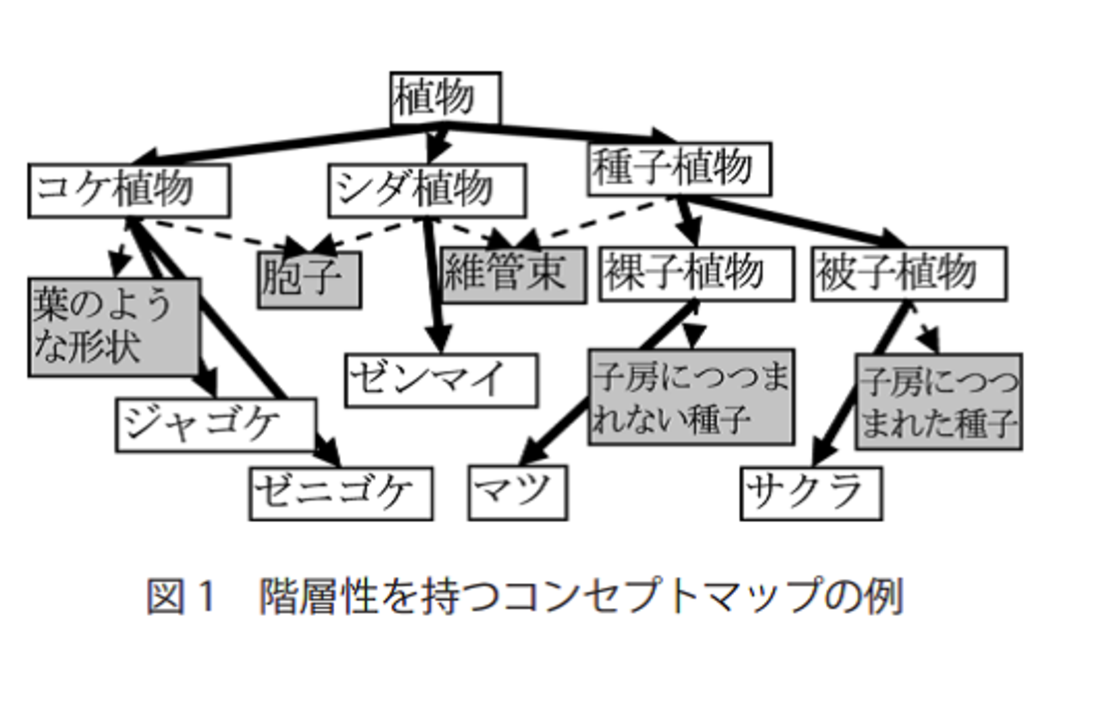
\includegraphics[width=8cm]{img/example_concept.eps}
\end{center}
\caption{コンセプトマップの例(出典: 誤りの可視化による階層構造の理解を指向したコンセプトマップ構築学習の支援環境 p.43 \cite{toumoto})}
\label{fig:example_concept}
\end{figure}

%
% キットビルド概念マップ
%
\chapter{キットビルド概念マップ}\label{chap:kitbuild}
\section{本章の概要}
本章では,キットビルド概念マップについて述べる.
キットビルド概念マップ\cite{kit}\cite{kit2}は,教授者が内容理解構造として作成した概念マップを分解・部品化して学習者に提供し,学習者は提供された部品を組立てることで概念マップを作成する.
組立てられた概念マップは,元の概念マップと重畳することで差分抽出が可能であり,また,複数のマップの重畳することによる集団としてのマップ作成も可能となっている.
これによりキットビルド概念マップは,内容理解構造の全般的で直接的な表出と,評価の自動化を実現する手段として使われている.

以降,キットビルド概念マップの特徴について述べる.

\section{キットビルド概念マップの特徴}
授業理解の過程において,Kiewra\cite{kiewra}やArmbruster\cite{armbruster}は情報の取得と情報館付けによる構造化の二つの過程より成立するとした.
構造化の過程が理解に対してより重要であると分析している.
また,情報の取得に失敗した場合,構造化では補完できない場合が多いため,構造化対象となる情報を学習者に明示的に示し,学習者には構造化に注力させるべきであるとしている.
キットビルド概念マップでは,構造化の対象となる情報を部品として学習者に提供することによって,構造化を保持しつつ情報取得失敗時による構造化失敗を回避できるという特徴がある.

また,教材内容の理解を教授者が概念マップとして明示的に記述することが求められる.
このことから概念マップとして表現できない深い学習内容に対しては表面的な理解に留まるような形でしか表現できない.
しかし,深い学習内容に至る前提としてキットビルド概念マップで表面的な内容理解で使用できるという点ではキットビルド概念マップの有用性は損なわれない.

同様にして,教授者が適切な概念マップを作成できるとは限らず,また,唯一の正解である概念マップを作製できるわけではない.
しかし,キットビルド概念マップでは,教授者が作成した概念マップと学習者が作成した概念マップを比較し,形成的評価・フィードバックを受ける,
すなわち学習者が作成した概念マップにおいて再構成ができていない部分や,同様の誤りが多い部分が存在した場合,教授者側が作成した概念マップに誤りがあると考えられるという点から概念マップの修正を重ねてより正確な概念マップを作成できる.

以上のようにしてキットビルド概念マップには,学習者には学習内容の構造化に注力させ,その構造化自体に誤りがあったとしてもそれを修正していけるような形で作成されているマップであると言える.

%
% 関連研究
%
\chapter{関連研究}\label{chap:refer}
\section{本章の概要}
本章では,本研究に関連する研究について述べる.
\ref{sec:concept_ref}節ではコンセプトマップを用いた研究について述べる.
\ref{sec:kasika_ref}節では学習成果の可視化に関する研究について述べる.
\ref{sec:my_thesis}節では,他研究と本研究にどのような違いがあるかを述べる.

\section{コンセプトマップを用いた研究}\label{sec:concept_ref}
コンセプトマップを用いた研究には,東本氏らの研究\cite{toumoto}と野村氏らの研究\cite{nomura_manabu}が挙げられる.
東本氏らの研究では,コンセプトマップを作成した学習者に対しフィードバックを返すことは重要であるが,決して容易ではないとしている.
第一に個別診断の困難性,第二に仮に診断をしても誤りをフィードバックしたとき,学習者の解答を否定し正解を提示する否定的フィードバックでは学習効果が低く,学習者はコンセプトマップの誤りを受け入れないか,なぜ誤りなのかを考えずに修正する可能性があり,自発的な誤り修正ができない点が挙げられる.
そこで,東本氏らは階層構造の理解の促進を目的とした学習者自身によるコンセプトマップの構築のためのシステム開発を行った.
特に,構築したコンセプトマップに対し,個別診断を行い,誤りがあれば誤りの可視化によるフィードバックを与えることとした.
東本氏らが提案した可視化手法は,各属性の意味を学習支援システムに組み込むため,汎用性が乏しいものとなった.
しかし,可視化を段階的に行うことにより,様々な階層性に対してもXMLや画像を用いれば可視化できるとしている.

野村氏の研究では,コンセプトマップはこれまで多くの教師が学校教育に取り入れており,コンセプトマップはある特定の学習過程において,教師と学習者が焦点化する必要のある少数のアイデアを明確にし,概念的意味を結びつける視覚的地図により,学習課題の達成後の図式的な要約を提供するものとしている.
しかし,コンセプトマップは学習中においても有効であるが最も友好的に利用できる可能なのは学習後の学習者の知識構成の表出であると主張している.
これはNovak\cite{concept}\cite{novak}が有意味学習の評価ツールとしてコンセプトマップが有効であるとしている点でも同様のことがいえるとしている.
そこで野村氏らはコンセプトマップを利用した学習ではなく,一定のまとまりのある学習内容を学習した結果をコンセプトマップを利用して評価することを想定とした,コンセプトマップを利用した学習評価支援システムを開発した.
このシステムでは,コンセプトマップの作成作業時間を短縮,管理を支援できる.

\section{学習成果の可視化に関する研究}\label{sec:kasika_ref}
学習成果の可視化に関する研究として,平塚氏ら\cite{hira}と手塚氏ら\cite{teduka}の研究が挙げられる.
平塚氏らの研究では,高等教育機関において学生自身が授業の学習成果を把握するものは,成績評定,GPA,資格取得などがあるとしているが,これらは授業単位を習得したという結果のみを計るものであり,学生にとって自分にどのような力が身についたのかわかりづらいとしている.
また,このことから学生は学習においての将来設計も難しくなり,授業の取り組みも消極的になるなど悪循環に陥ってしまう.
そこで,平塚氏らは学習成果の到達度を可視化し,学生に分かりやすい形で提示し自己効力感を得て学習意欲向上のために,教務システムとeポートフォリオを連携した学習成果可視化システムを構築した.
すでに同様のシステムを独自開発している事例はあるが,オープンソースのシステムを用いて構築し,公開・フィードバックする点が研究の意義としている.

手塚氏らの研究では,高等教育における振り返りは他者と関わりあいながら自主的に学び続けるために必要な能力として注目されているとし,構成主義的な学習観において教員が何を教えるかから学習者が何を学び取るかへと視点の転換が主張されていることから,学習中に期待通り成果が得られたのかどうかを常に振り返り,成功または失敗の要因を学習者が認識することが重要であるとしている.
しかし,全学習者が適切に振り返りを行えるとは限らないため,平塚氏らは振り返りの質的向上を目的とし,期末試験の予測得点と学習者データの可視化による振り返り支援システムを提案・開発した.
振り返りシステムでは,基礎数学の振り返りシートを分析し,eラーニングのヒント閲覧回数,eラーニングの学習時間,Vマーク式学習法におけるVの数が理解度の向上に結びつく振り返りに役立つことが考えられため,それらを折れ線グラフで時系列順に可視化するシステムを作成した.
これにより学習者は可視化機能を用いて学習でき,さらに各学習者がどのような学習データを見ながら振り返りを行っているのかというログが収集できる.

\section{本研究の特徴}\label{sec:my_thesis}
いままで上げてきた研究はどれも実際の授業の中でコンセプトマップや学習者の学習進捗を可視化しているものが多い.
一方,本研究では,eラーニングで学習する学習者に重きを置いている.
eラーニングは確かに授業の一環として用いられることもあるが,基本的には学習者一人で課題をこなしていくものが多い.
また,eラーニングにおけるフィードバックは否定的フィードバックが多く,何故間違えたのかという思考に至る可能性が低くなる.
加えて,今までの研究成果物はそのシステム上でのみ動作する物が多い.
本研究ではeラーニング上で学習する学習者に対して指導者が直接かかわらずとも学習者自身だけで,自身の学習理解度を把握し,学習目標を設定できる.
また,本システムはグラフデータの作成,削除や可視化に至るデータ取得に関して全てAPI化して実装している.
このことにより,本システムの可視化表現方法は本システムのみで使用できる機能となっているが,コンセプトマップの情報をグラフデータに変換し保存,削除,またデータ呼び出しに関してはAPIを通じて実行できる.
このことから,可視化に至るまでのデータ取得は任意のアプリケーションでも実施できるため,様々なeラーニングシステムで本システムの機能を実行できる.




%
% システム要件
%
\chapter{システム要件}\label{chap:content}
\section{本章の概要}
本章では,本システムの概要について述べる.
本システムは,eラーニングで学習している学習者を対象としたシステムで,コンセプトマップを利用して学習者が学習目標を設定する場合に本システムを利用することを想定している.
本システムを利用して学習を進めることで,コンセプトマップにより自身の学習分野に対する構造的な理解を促進できるだけでなく,自身が進めている学習分野の主観的な知識獲得量を客観的に把握することが出来るため,学習目標を設定しやすくなる.

\ref{sec:kousei}節では,本システムの構成について述べる.
\ref{sec:env}節では,本システムの開発環境について述べる.
\ref{sec:about_system}節では,本システムにおける各機能の概要について述べる.
\ref{sec:futan}節では,本システムの運用における指導者の負担について述べる.

\section{本システムの構成}\label{sec:kousei}
本システムの構成を図\ref{fig:kousei}に示す.
本システムは,学習者がインターネットを通じて本システムのWebアプリケーションに接続することによってコンセプトマップを作成し学習を進めることができる.
本システムはすべての開発環境をDockerを用いて作成しているため,Dockerを使用できる環境であればどこでも本システムを実行することが可能である.

本システムで利用可能な学習教材は,その学習分野において教材提供者が階層構造を持つと判断した学習教材であれば利用可能である.
コンセプトマップを作成するにあたって,本システムではグラフデータベースを用いてコンセプトマップにおけるノードやリンク,リンクキーワードをグラフデータベースにおけるノード,エッジ,プロパティに変換することによってグラフデータベースにコンセプトマップのデータを保存し,その後グラフデータベースを可視化するライブラリを用いてコンセプトマップを閲覧,作成できる機能を作成した.
本システムを利用した学習手順として,学習者は指導者が作成した学習コンテンツを学び,そのフィードバックとして各問題がどのような学習分野となるのか教授してもらう.
その後,本システムを用いてそれぞれの学習分野をコンセプトマップを用いてどのような階層構造になっているのかを予測しながらコンセプトマップを作成する.
最後に本システムが指導者から入力された学習分野に対する階層構造のデータからコンセプトマップを自動的に作成する.
これにより学習者は,自身が作成したコンセプトマップと,自動的に作成されたコンセプトマップとを比較することにより,学習分野における自身の階層構造に対する理解を深めることができる.
加えて本システムではコンセプトマップのノードにおいて学習者の問題の回答情報から点数によってノードの背景色を表示できる.
これにより学習者は対象学習分野について,主観的に考えていた学習理解度と実際のテストの点数による学習理解度をはっきりと視覚的に確認でき,自分は特定分野においてしっかり学修できていたと思っていたが,実際はあまり理解できてきなかったという勘違いを正すことができる.
\begin{figure}[htbp]
\begin{center}
\includegraphics[width=10cm]{img/kousei.eps}
\end{center}
\caption{システム構成}
\label{fig:kousei}
\end{figure}

\section{開発環境}\label{sec:env}
本システムは,コンテナ仮想化プラットフォームであるDockerを基盤として開発している.
指導者は,本システムの運用Webサーバが内包されたDockerイメージを自身のPC上にインポートして学習用コンテナを生成することで,Webアプリケーションを実行でき,学習者に対してコンセプトマップを用いた学習を実施できる.
また,本システムにおけるグラフデータベースであるNeo4jとPythonのWebフレームワークの一つであるFlaskを用いることによりグラフデータベースとコンセプトマップのデータ変換部をAPIを用いて作成していることにより,様々なプラットフォームで本システムのグラフデータべース+コンセプトマップという学習環境を利用する事が可能である.
以下に,本システムの利用にあたって指導者が実行しなければならないDockerコマンドを一覧に示す.

\begin{itemize}
    \item docker-compose up -d --build\\
    - 指導者のPC上に本システムのDockerイメージをインポートし実行する
    
    \item docker-compose down -v\\
    - 本システムに何か変更を加えた際にコンテナを停止させるためのコマンド

    \item docker system prune\\
    - 本システムに何か変更を加えた際にコンテナに残っているキャッシュを削除するためのコマンド
    
\end{itemize}


\section{本システムにおける各機能の概要}\label{sec:about_system}
本システムは大きく分けて3つの機能によって成り立っている.
それは,グラフデータ管理機能,グラフデータ入力補助機能,グラフデータ可視化機能の3つの機能である.
それぞれの機能について\ref{subsec:kanri}節,\ref{subsec:hojo}節,\ref{subsec:kasi}節で説明する.

\subsection{グラフデータ管理機能}\label{subsec:kanri}
グラフデータ管理機能は,学習者と指導者のグラフデータを管理する機能で,クライアントのフォームから入力されたコンセプトマップの親子に関するデータをAPIを用いてグラフデータへと変換しグラフデータベースへとデータを登録する.
また,クライアントからグラフデータを要求された場合,グラフデータをAPIを用いてJSON形式で返答する.

グラフデータ管理機能が使用するAPIは以下のとおりである.

\begin{itemize}
    \item /create/json \\
    - 与えられたJSON形式のデータをグラフデータベースで利用できるJSON形式のデータに変換し,データを登録しその結果をJSON形式で返答する.

    \item /get/all\_graphs \\
    - グラフデータベースに登録されているすべてのグラフデータをJOSN形式で返答する.

    \item /create/score \\
    - 指定されたユーザと教科の点数登録を行う.

    \item /get/score \\
    - 指定された教科に紐づくすべての点数を返答する.

    \item /get/score/\<username\> \\
    - 指定されたユーザに関する教科の得点を返答する.

    \item /get/subject/\<subject\> \\
    - 指定されたユーザが受験した科目と点数を返答する.

    \item /delete/\<string:node\_name\> \\
    - 指定されたノードを削除する.

    \item /delete/all \\
    - すべてのノードを削除する.
    
\end{itemize}

これらのAPIを利用することにより本システムはグラフデータベースとコンセプトマップを紐づけて利用している.
\newpage

\subsection{グラフデータ入力補助機能}\label{subsec:hojo}

グラフデータ入力補助機能のGUIを図\ref{fig:hojo}に示す.

\begin{figure}[htbp]
\begin{center}
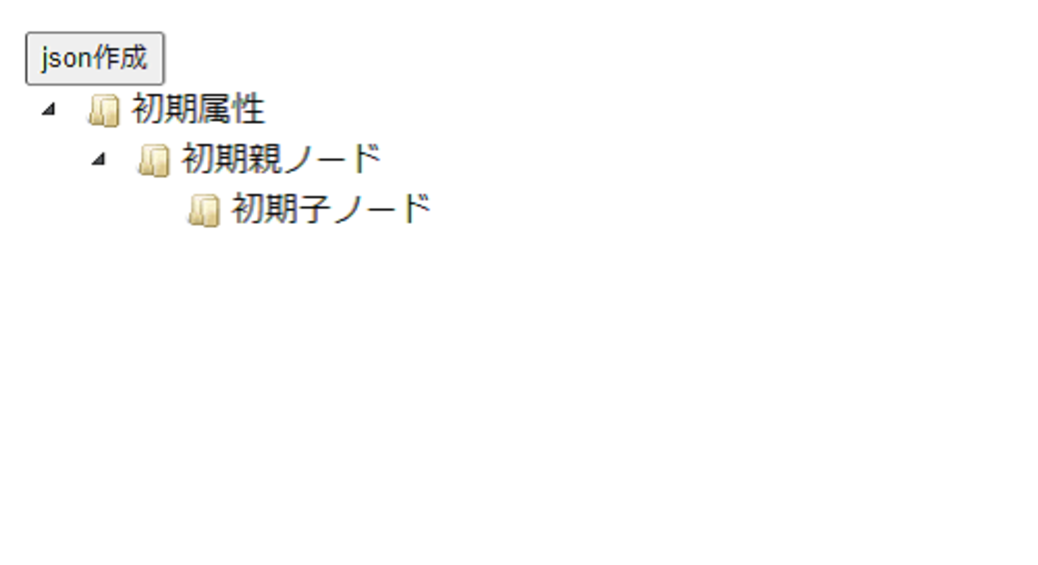
\includegraphics[width=10cm]{img/hojo.eps}
\end{center}
\caption{グラフデータ入力補助機能初期状態}
\label{fig:hojo}
\end{figure}

図\ref{fig:hojo}は初期状態で,図のような木構造な入力フォームを提示する.
初期属性とは第\ref{chap:conceptmap}章の図\ref{fig:example_concept}で示した植物に該当する.
初期親ノードは被子植物,初期子ノードはサクラに該当する.

各々の階層は図\ref{fig:hojo_change_name}のようにして各ノードを右クリックすることによりメニューが表示される.

\begin{figure}[htbp]
\begin{center}
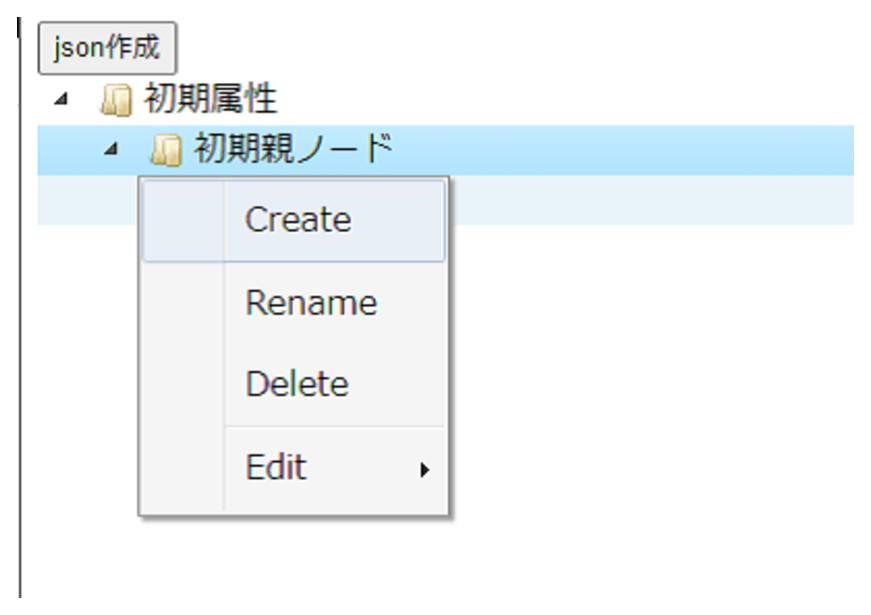
\includegraphics[width=10cm]{img/hojo_change_name.eps}
\end{center}
\caption{グラフデータ入力補助機能編集状態}
\label{fig:hojo_change_name}
\end{figure}

\subsection{グラフデータ可視化機能}\label{subsec:kasi}


\section{本システムの運用における指導者の負担}\label{sec:futan}




%
% 学習者理解度可視化システム
%
\chapter{学習者理解度可視化システム}\label{chap:system}
\section{本章の概要}
本章では,学習者理解度可視化システムとしてのシステムにおける具体的な実行手順と,それぞれの機能についての詳細について述べる.

\section{システム実行手順の流れ}
\subsection{前提条件}
本システムを実行する前に満たすべき前提条件を示す.
まず,本システムは全てDocker上で動作するため,Dockerを使用できるPC上でのみ動作する.
そのPCの必要最低動作環境を表\ref{tab:docker_env}に示す.

\begin{table}[htb]
    \centering
    \caption{Dockerのシステム要件}
    \label{tab:docker_env}
    \begin{tabular}{|c|c|}  \hline
        \multirow{5}{*}{Windows} & Windows 10 64 ビット:Pro、Enterprise、Education(ビルド 15063 以上) \\
		              & Hyper-V と Windows コンテナ機能の有効化 \\ 
                      & 64 ビット SLAT (Second Level Address Translation) 対応プロセッサ \\ 
                      & 4GB システムメモリ \\ 
                      & BIOS レベルでのハードウェア仮想化の有効化 \\ \hline
        \multirow{2}{*}{Intel チップの Mac} & macOS はバージョン 10.15 またはそれ以降 \\
        & 最小 4GB の メモリ RAM \\ \hline
        Apple silicon の Mac & Rosetta 2 のインストール \\ \hline
        \multirow{7}{*}{Linux系} & 仮想化のために、 64-bit カーネルと CPU のサポート \\
        & KVM 仮想化のサポート \\ 
        & QEMUバージョン5.2以上 \\
        & systemd init システム \\ 
        & Gnome または KDE デスクトップ環境 \\ 
        & 最小 4GB の メモリ RAM \\
        & ユーザ名前空間で ID マッピングの設定を有効化 \\ \hline
    \end{tabular}
\end{table}

%
% 評価実験
%
\chapter{評価実験}\label{chap:experiment}
\section{本章の概要}
本章では,開発したシステムの評価実験とその考察について述べる.
そして本研究では,学習者が座学における学習目標設定方法による学習と本システムのグラフデータ可視化機能を用いた学習目標設定方法による学習を比較し,
有用性を検証するための事前事後テストによる評価実験とアンケートによる利用評価実験を実施した.

\section{座学と比較した本システムによる学習の有用性検証実験}
実験では,基本情報技術者試験の午前試験\cite{gozen}を基にした,事前テスト事後テストによる座学と比較した本システムによる
学習の有用性を検証した.

\subsection{実験対象者}
実験対象者は,情報学科の学生と情報学科を卒業した大学院生(4年生:4名,修士1年生:7名,修士2年生:5名)の16名を実験協力者とした.
当学科では,3年生までにプログラミングは勿論ながら様々な情報学に関しての講義があるため,基本情報処理技術者試験の午前試験に関する知識も備えている.

\subsection{実験準備}
本実験を実施するにあたり,基本情報技術者試験の午前試験に関する事前テスト・事後テストを用意した.
学習教材としては事前テストに解説を付属させておりそれを学習教材とした.

事前テスト,事後テストはともに10点満点として,事前テスト・事後テストは同レベルの別の問題を使用した.
事前テストと事後テストはGoole From上で解答してもらった.
事前テストの内容を図\ref{fig:jizen1}~図\ref{fig:jizen6}に示す.
事後テストの内容を図\ref{fig:jigo1}~図\ref{fig:jigo6}に示す.
学習教材の例を図\ref{fig:kyozai1},図\ref{fig:kyozai2}に示す.

\begin{figure}[htbp]
\begin{center}
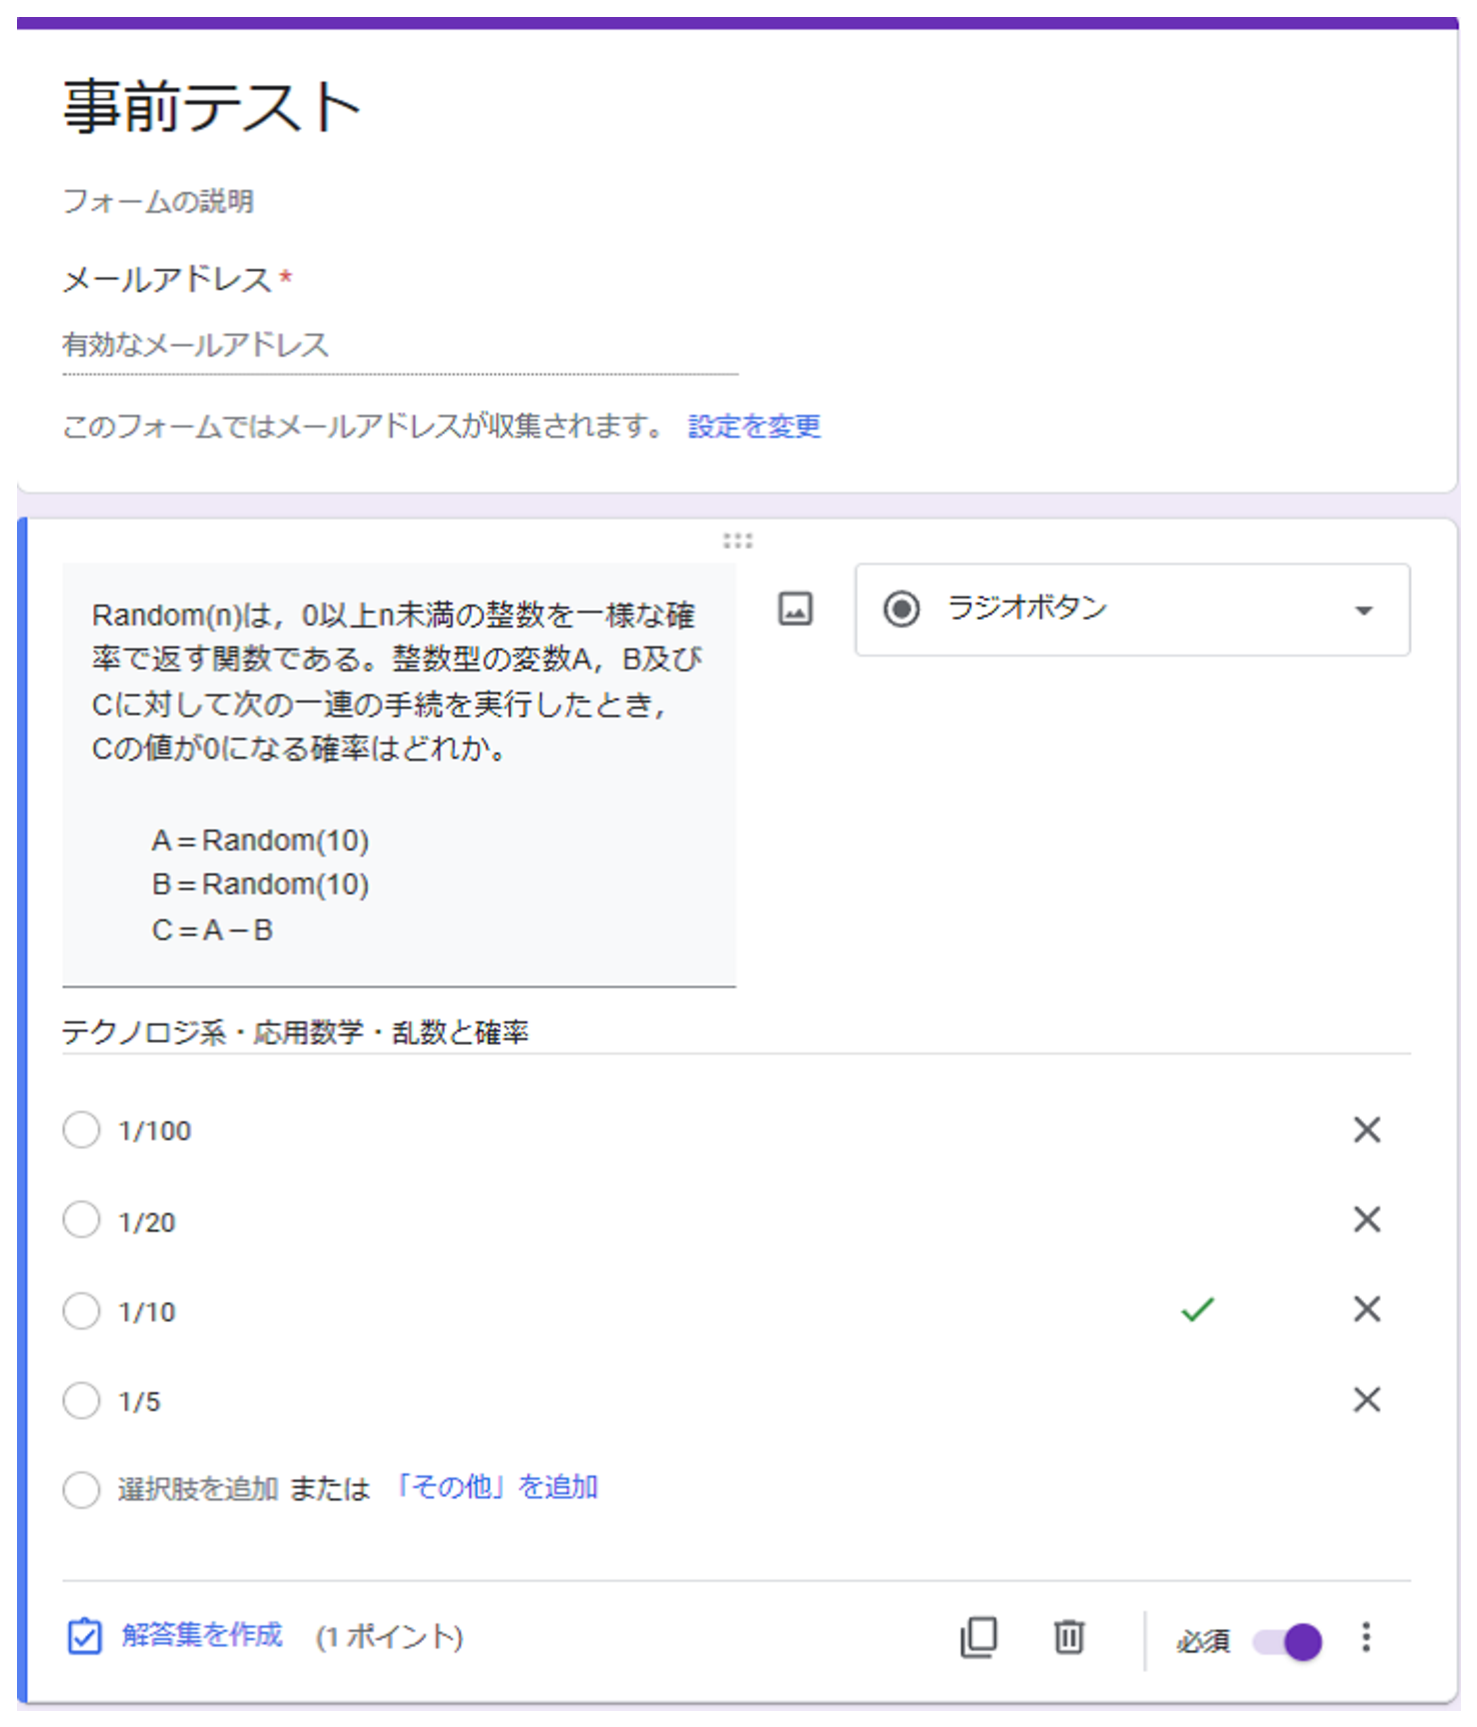
\includegraphics[width=13cm]{img/jizen1.eps}
\end{center}
\caption{事前テスト問題例1}
\label{fig:jizen1}
\end{figure}

\begin{figure}[htbp]
\begin{center}
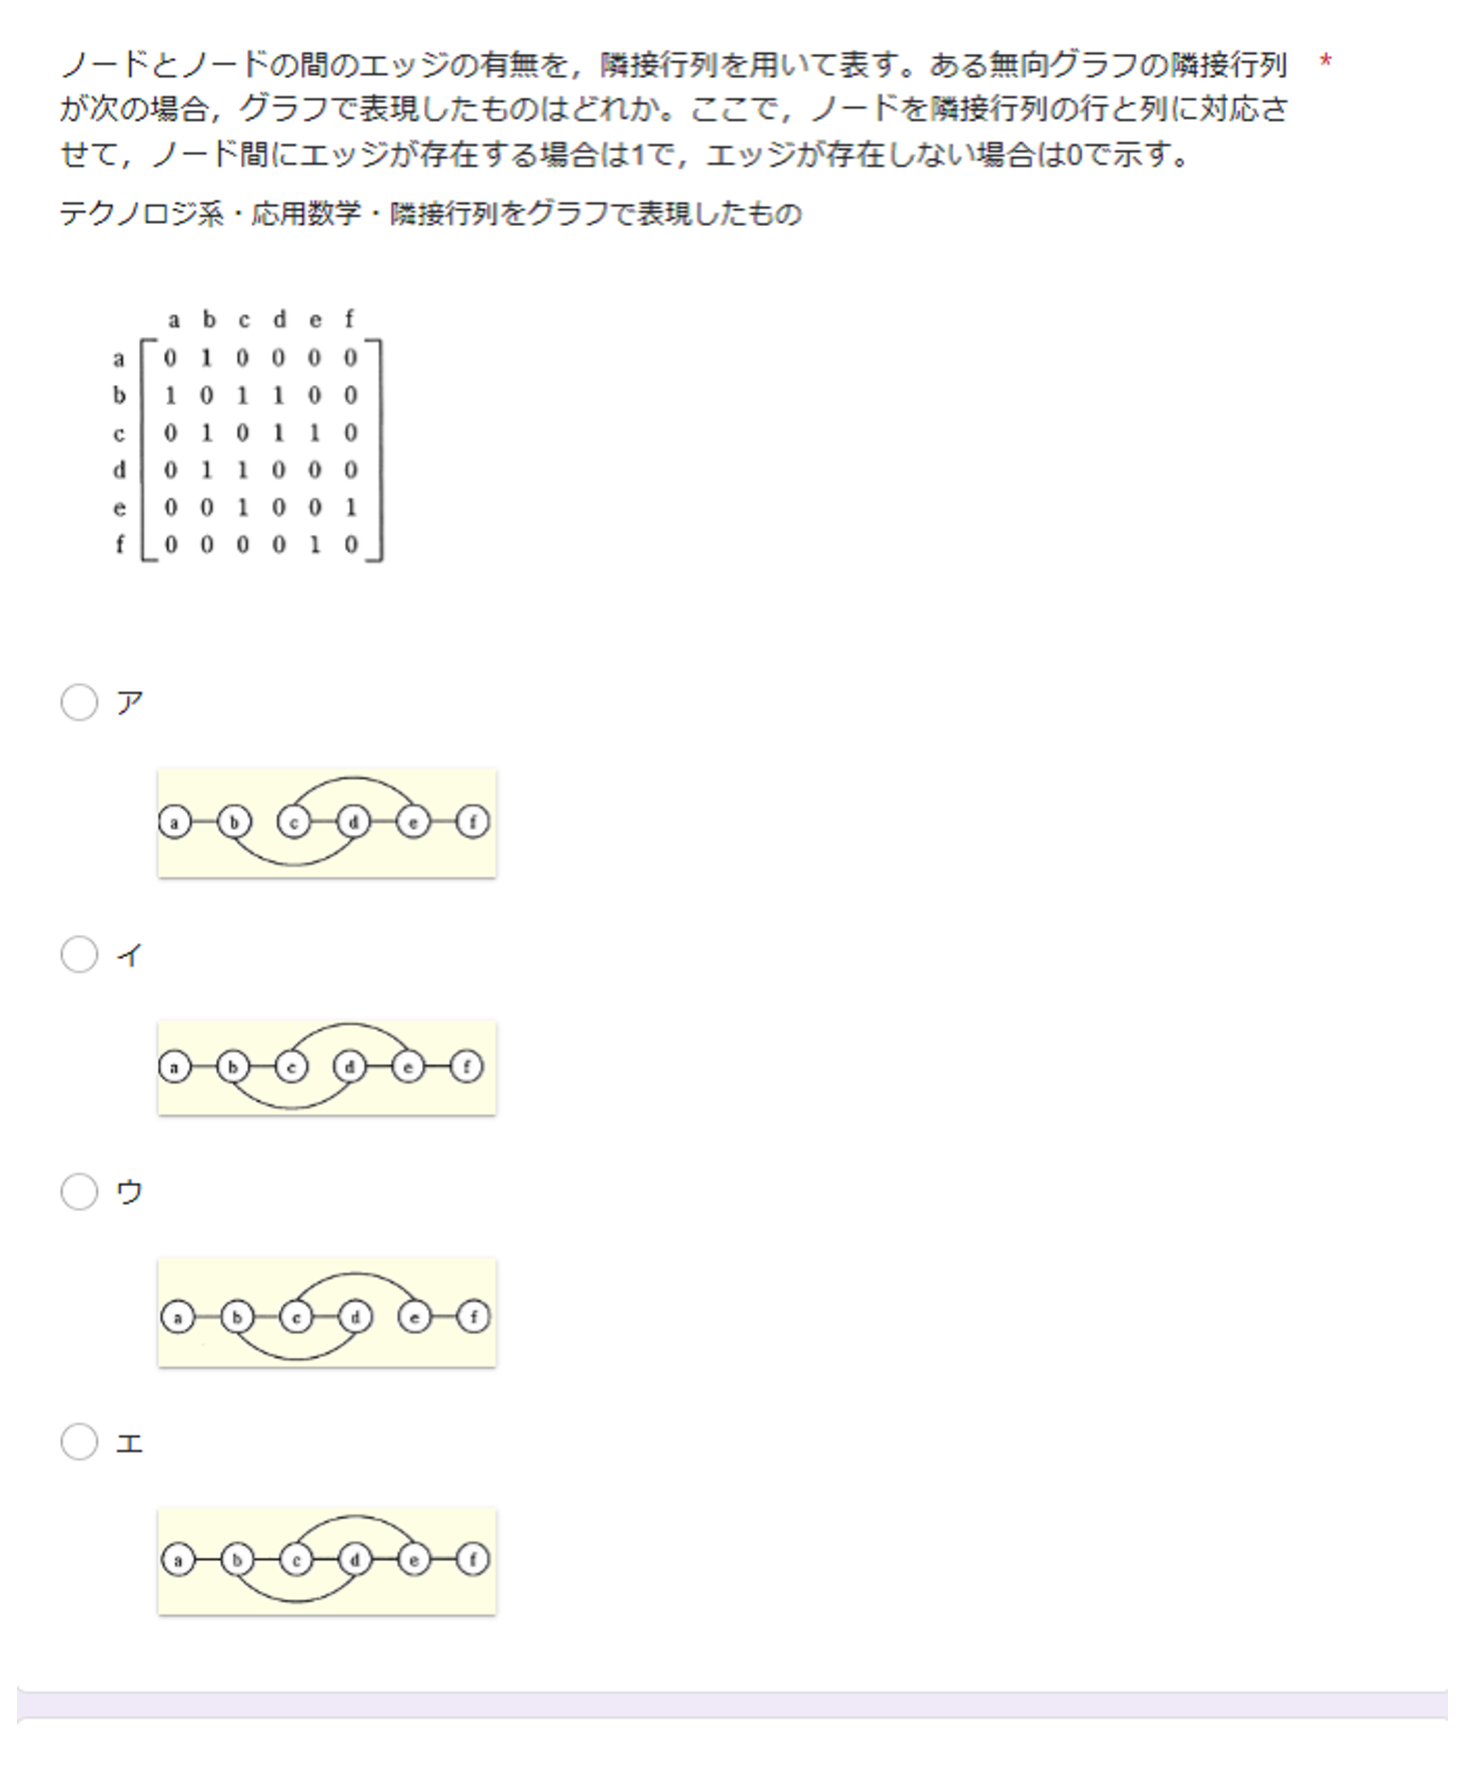
\includegraphics[width=16cm]{img/jizen3.eps}
\end{center}
\caption{事前テスト問題例2}
\label{fig:jizen3}
\end{figure}

\begin{figure}[htbp]
\begin{center}
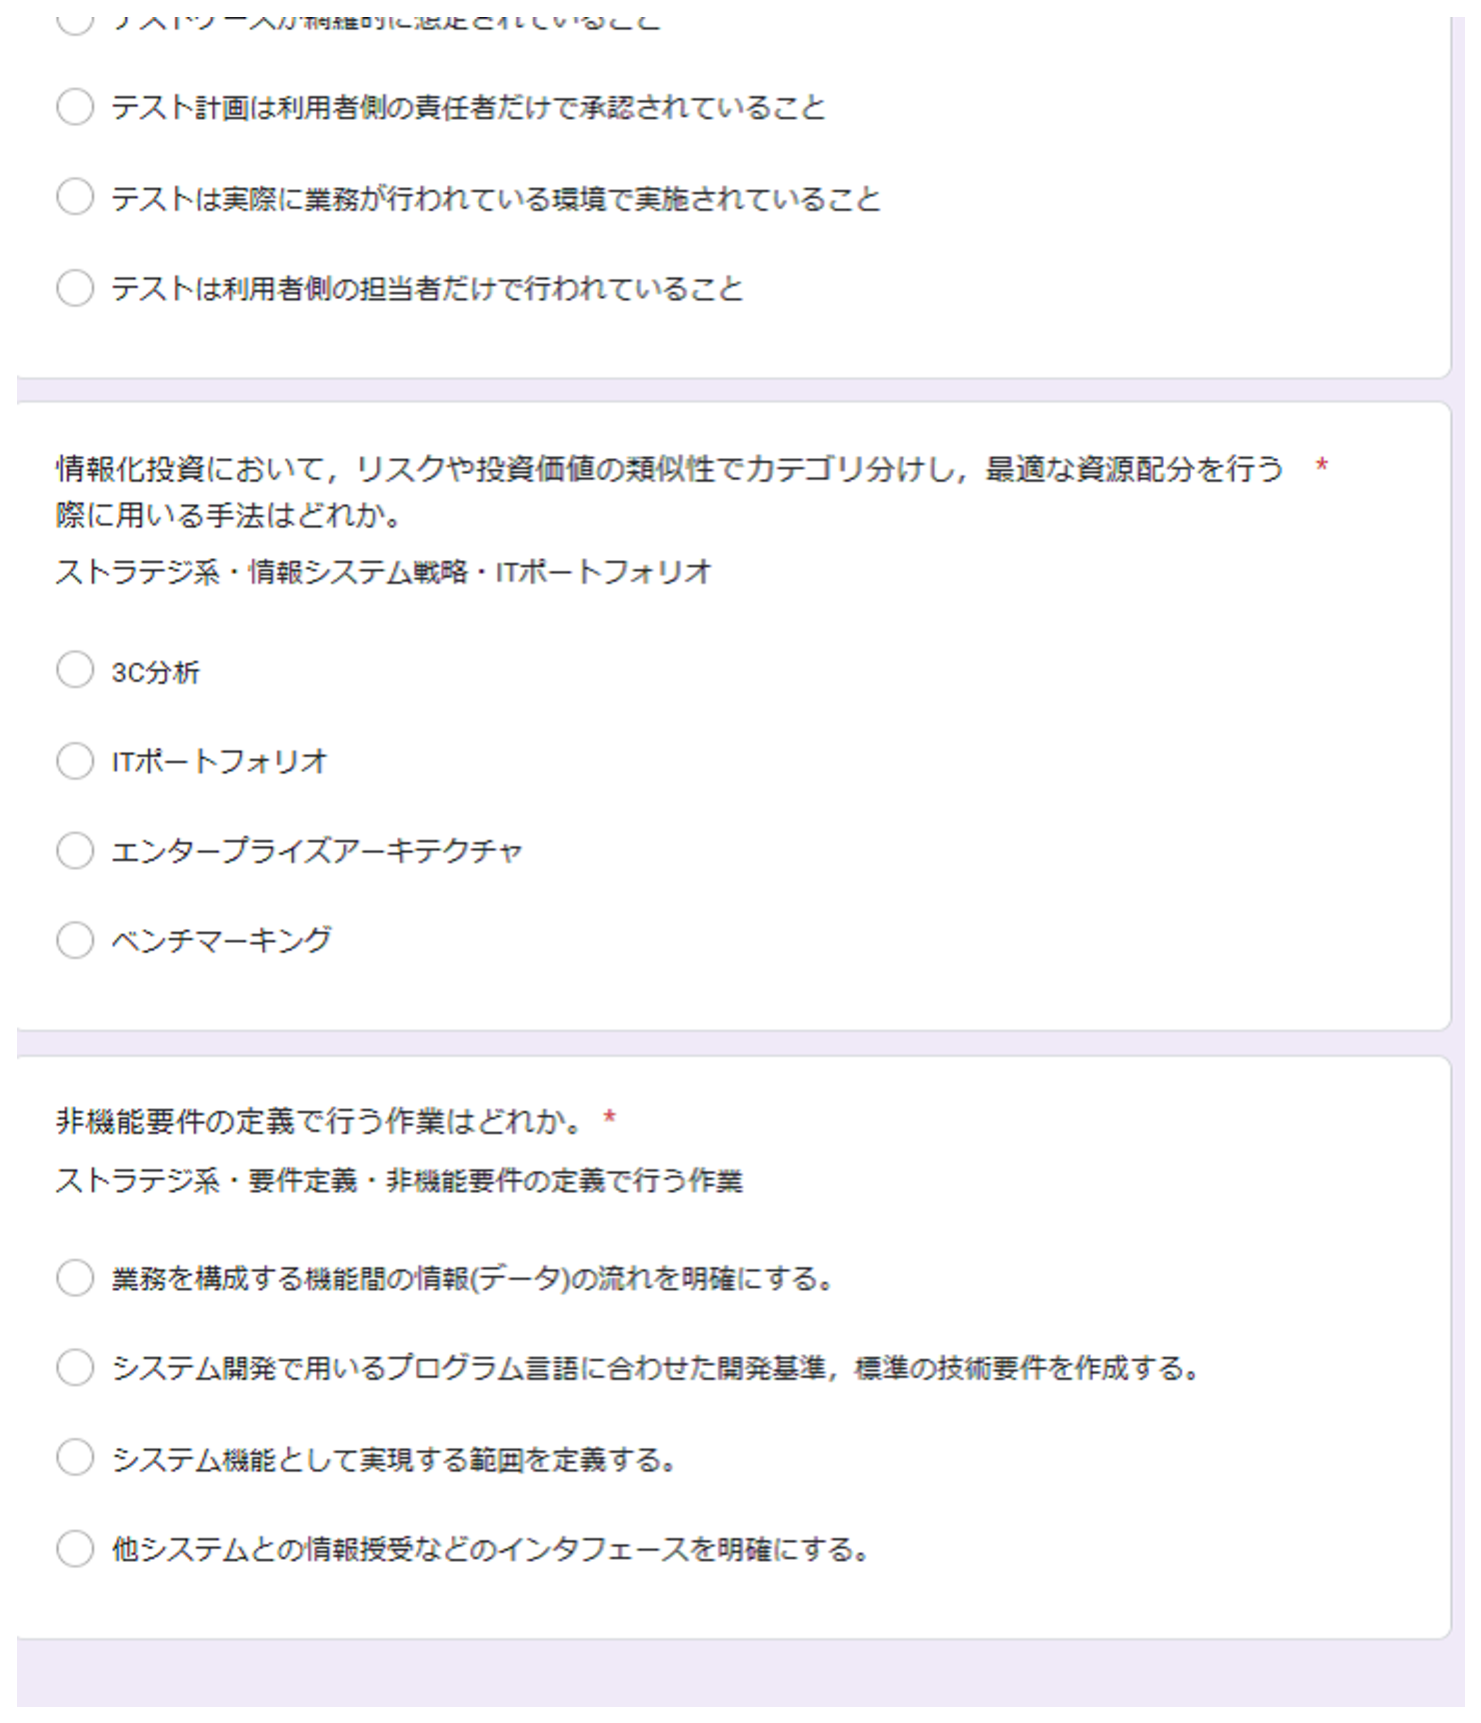
\includegraphics[width=16cm]{img/jizen6.eps}
\end{center}
\caption{事前テスト問題例3}
\label{fig:jizen6}
\end{figure}

\begin{figure}[htbp]
\begin{center}
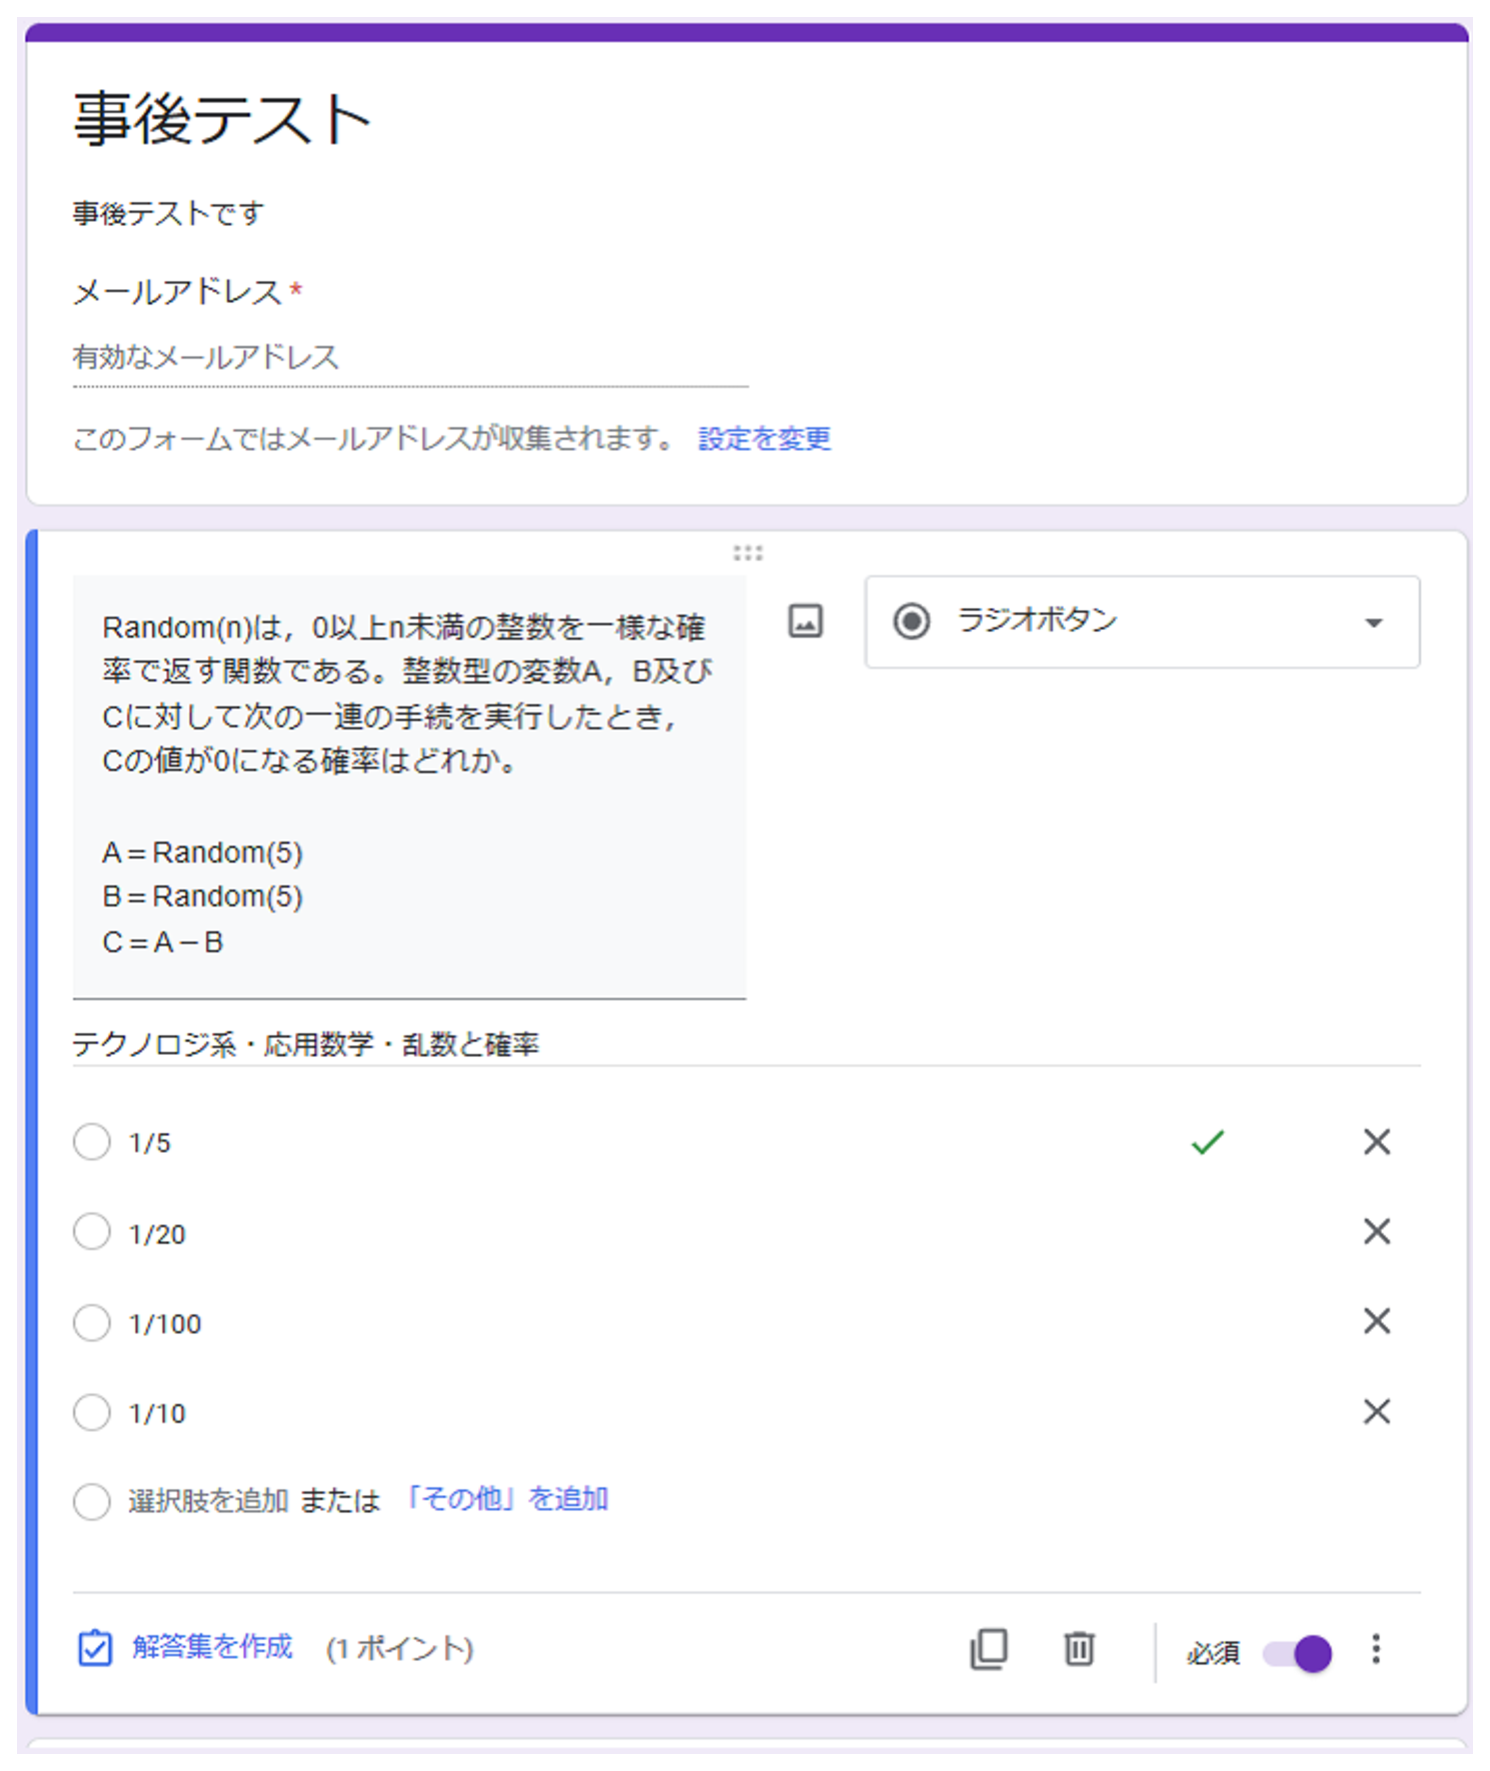
\includegraphics[width=16cm]{img/jigo1.eps}
\end{center}
\caption{事後テスト問題例1}
\label{fig:jigo1}
\end{figure}

\begin{figure}[htbp]
\begin{center}
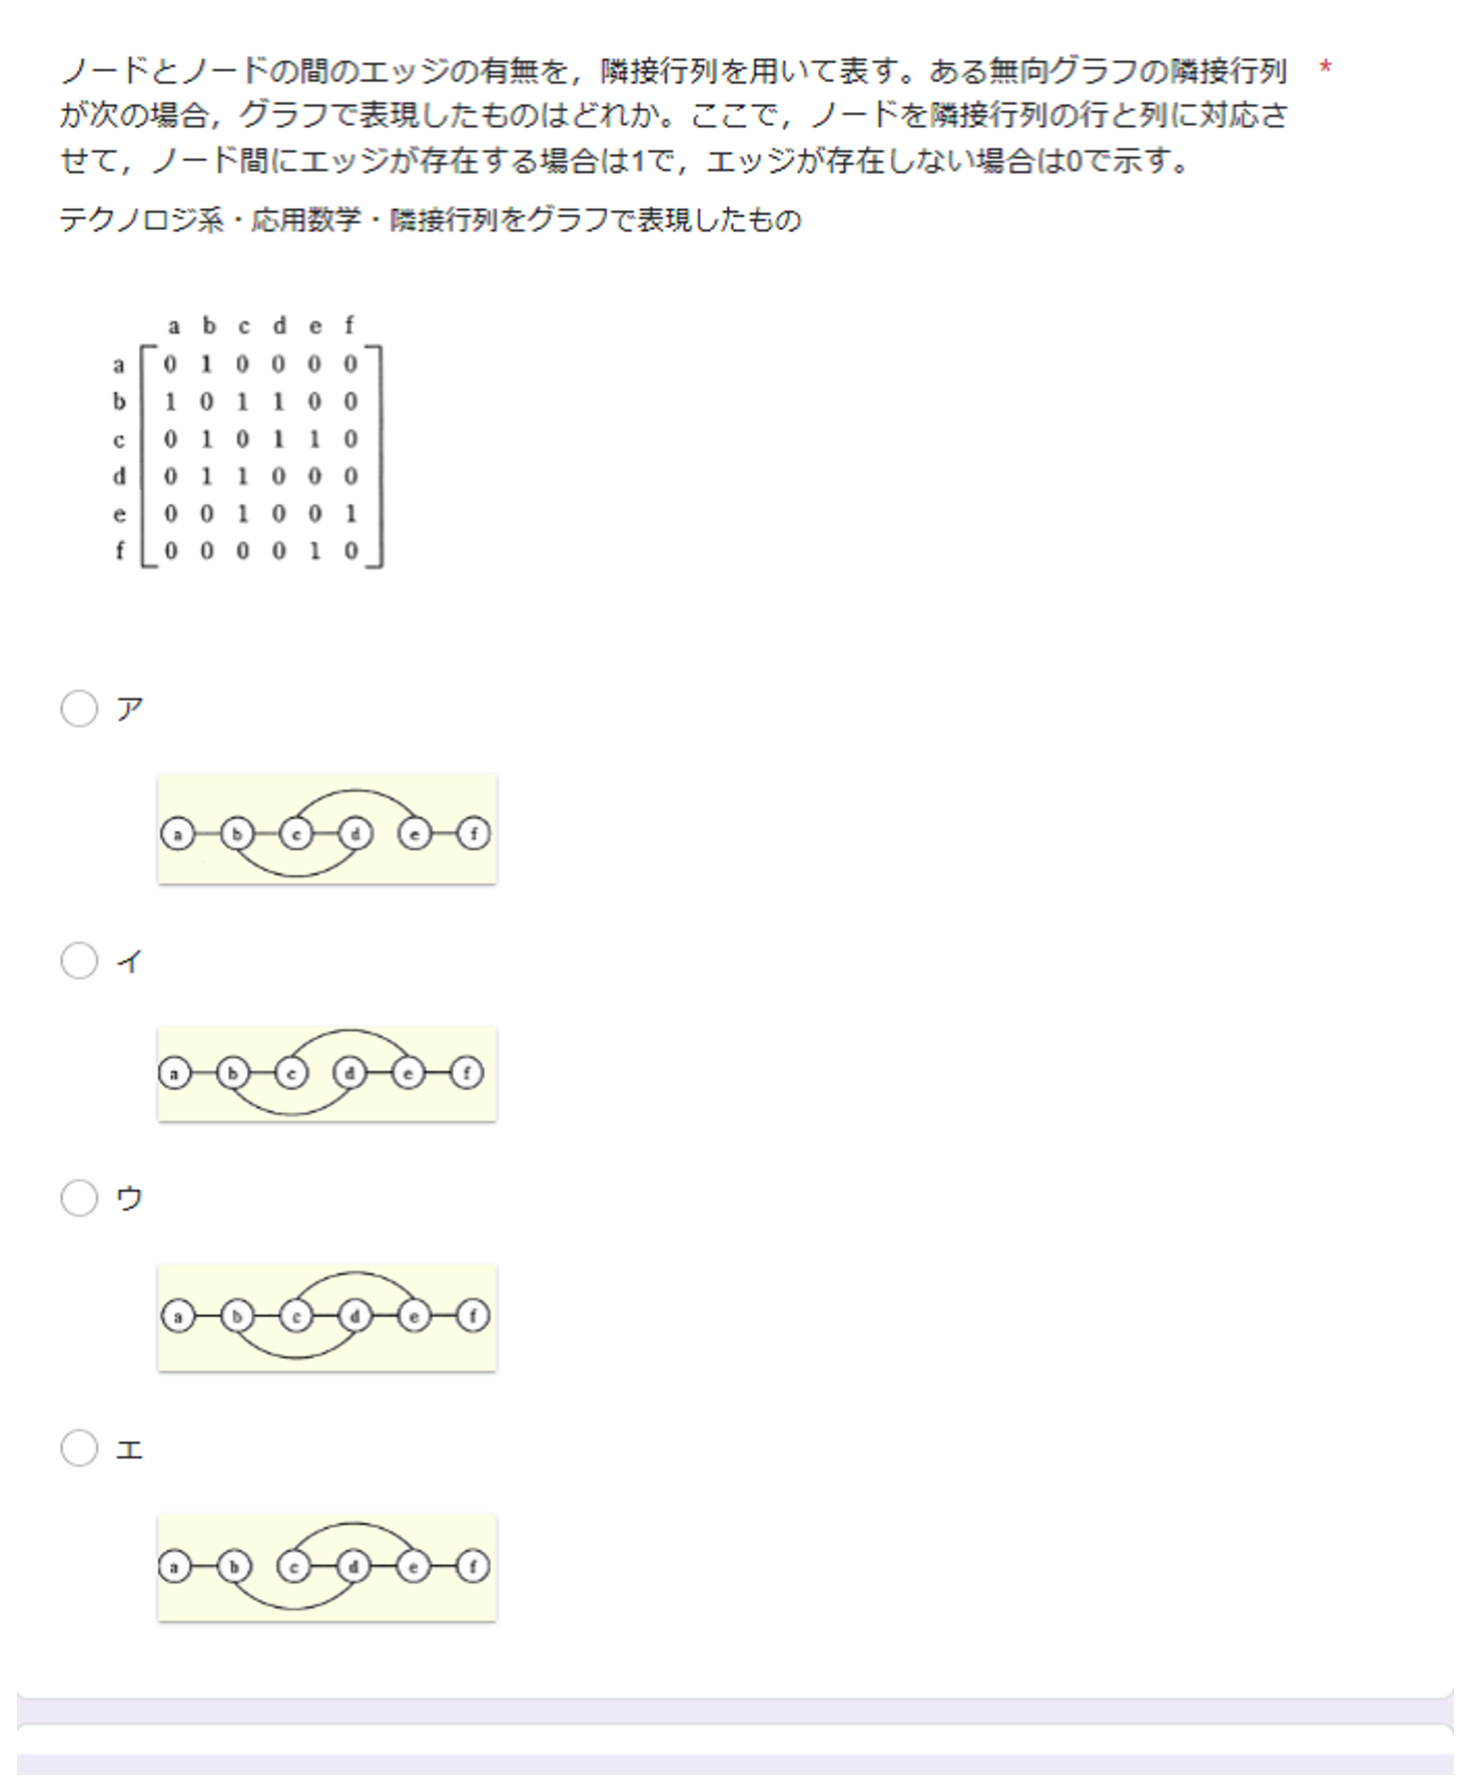
\includegraphics[width=16cm]{img/jigo3.eps}
\end{center}
\caption{事後テスト問題例2}
\label{fig:jigo3}
\end{figure}

\begin{figure}[htbp]
\begin{center}
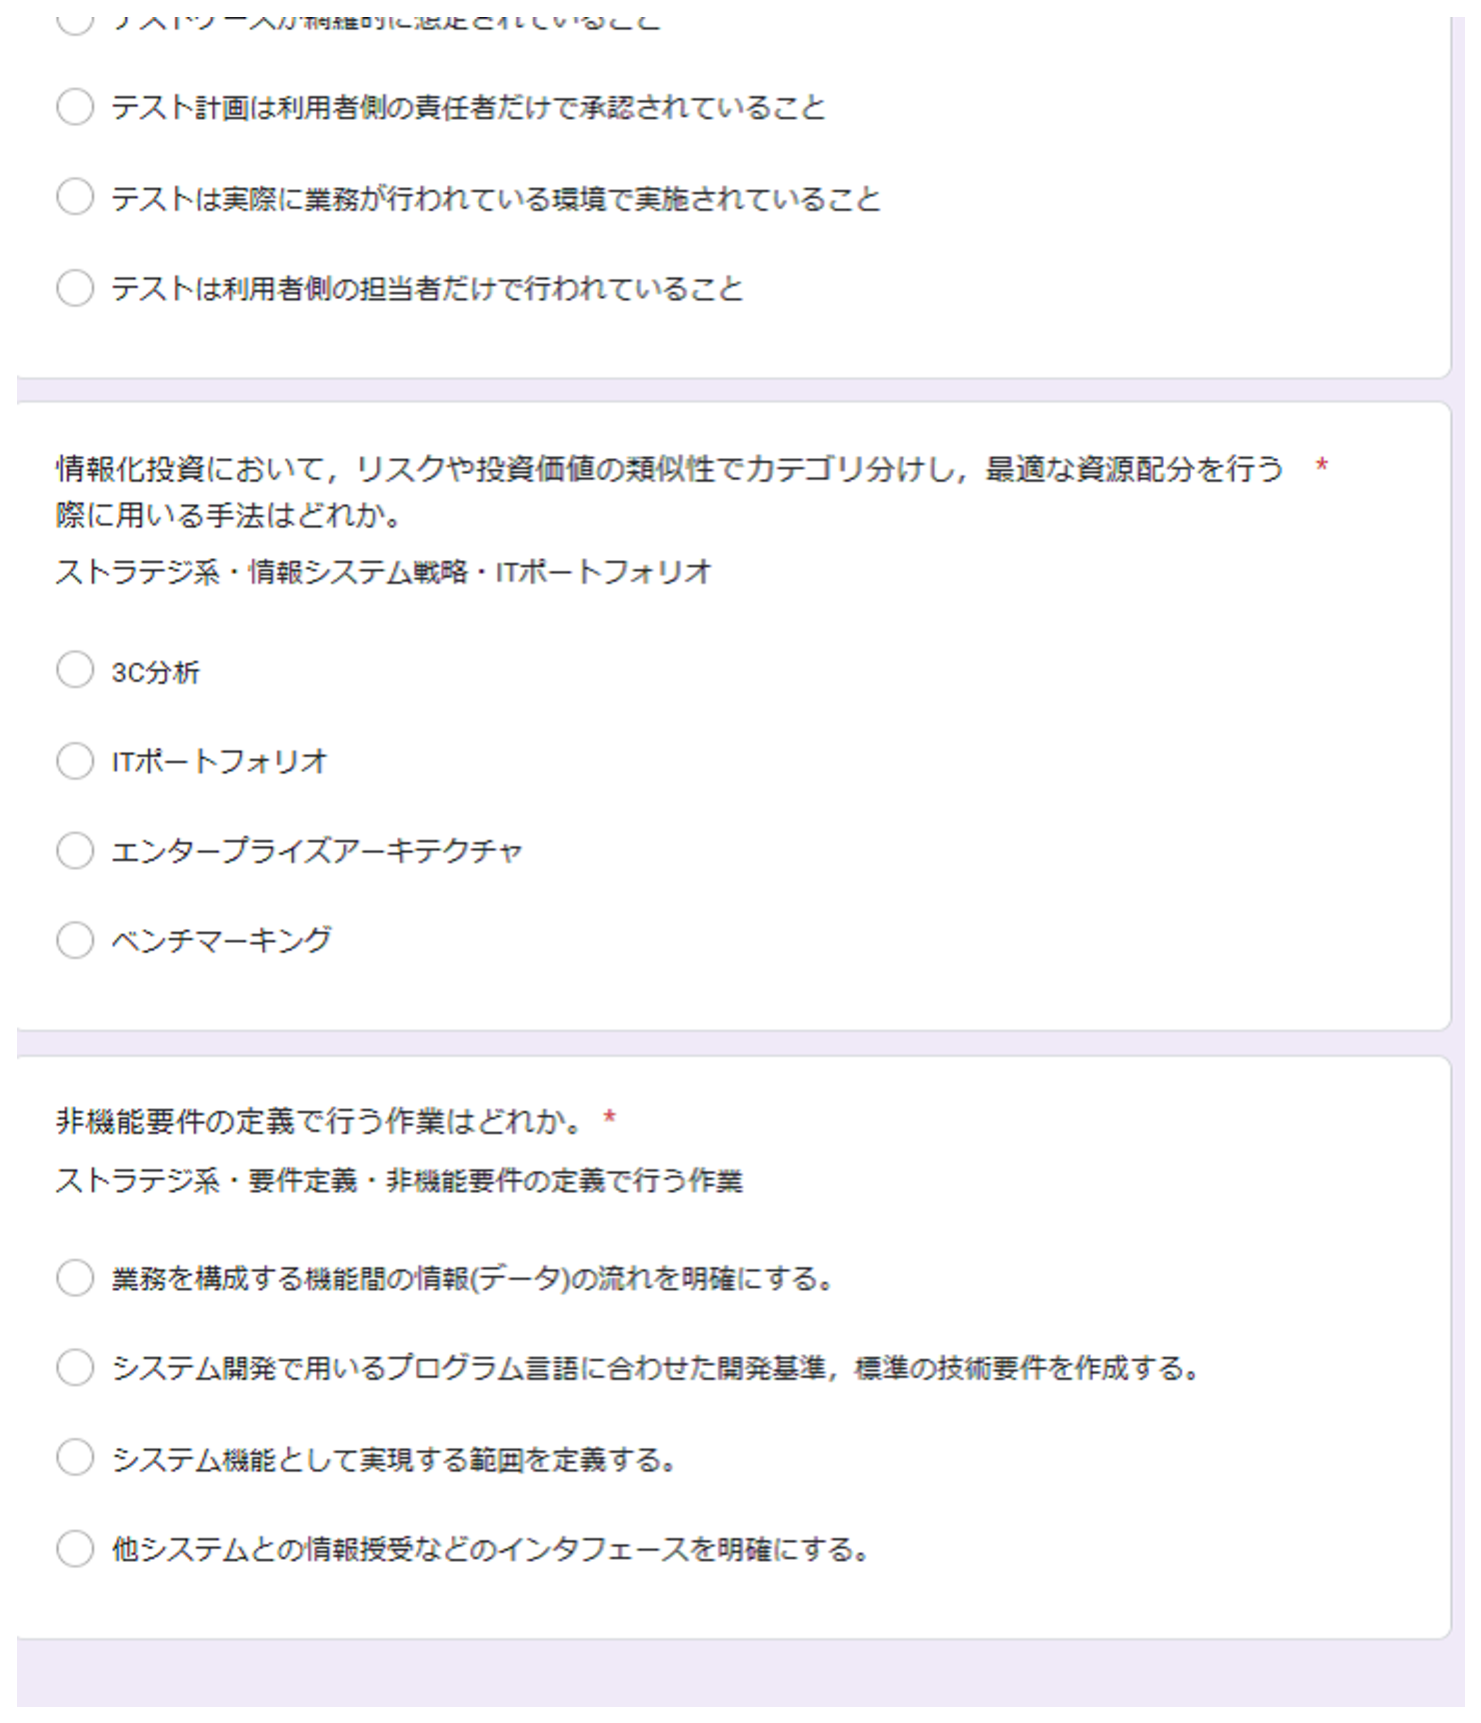
\includegraphics[width=16cm]{img/jizen6.eps}
\end{center}
\caption{事後テスト問題例3}
\label{fig:jigo6}
\end{figure}

\begin{figure}[htbp]
\begin{center}
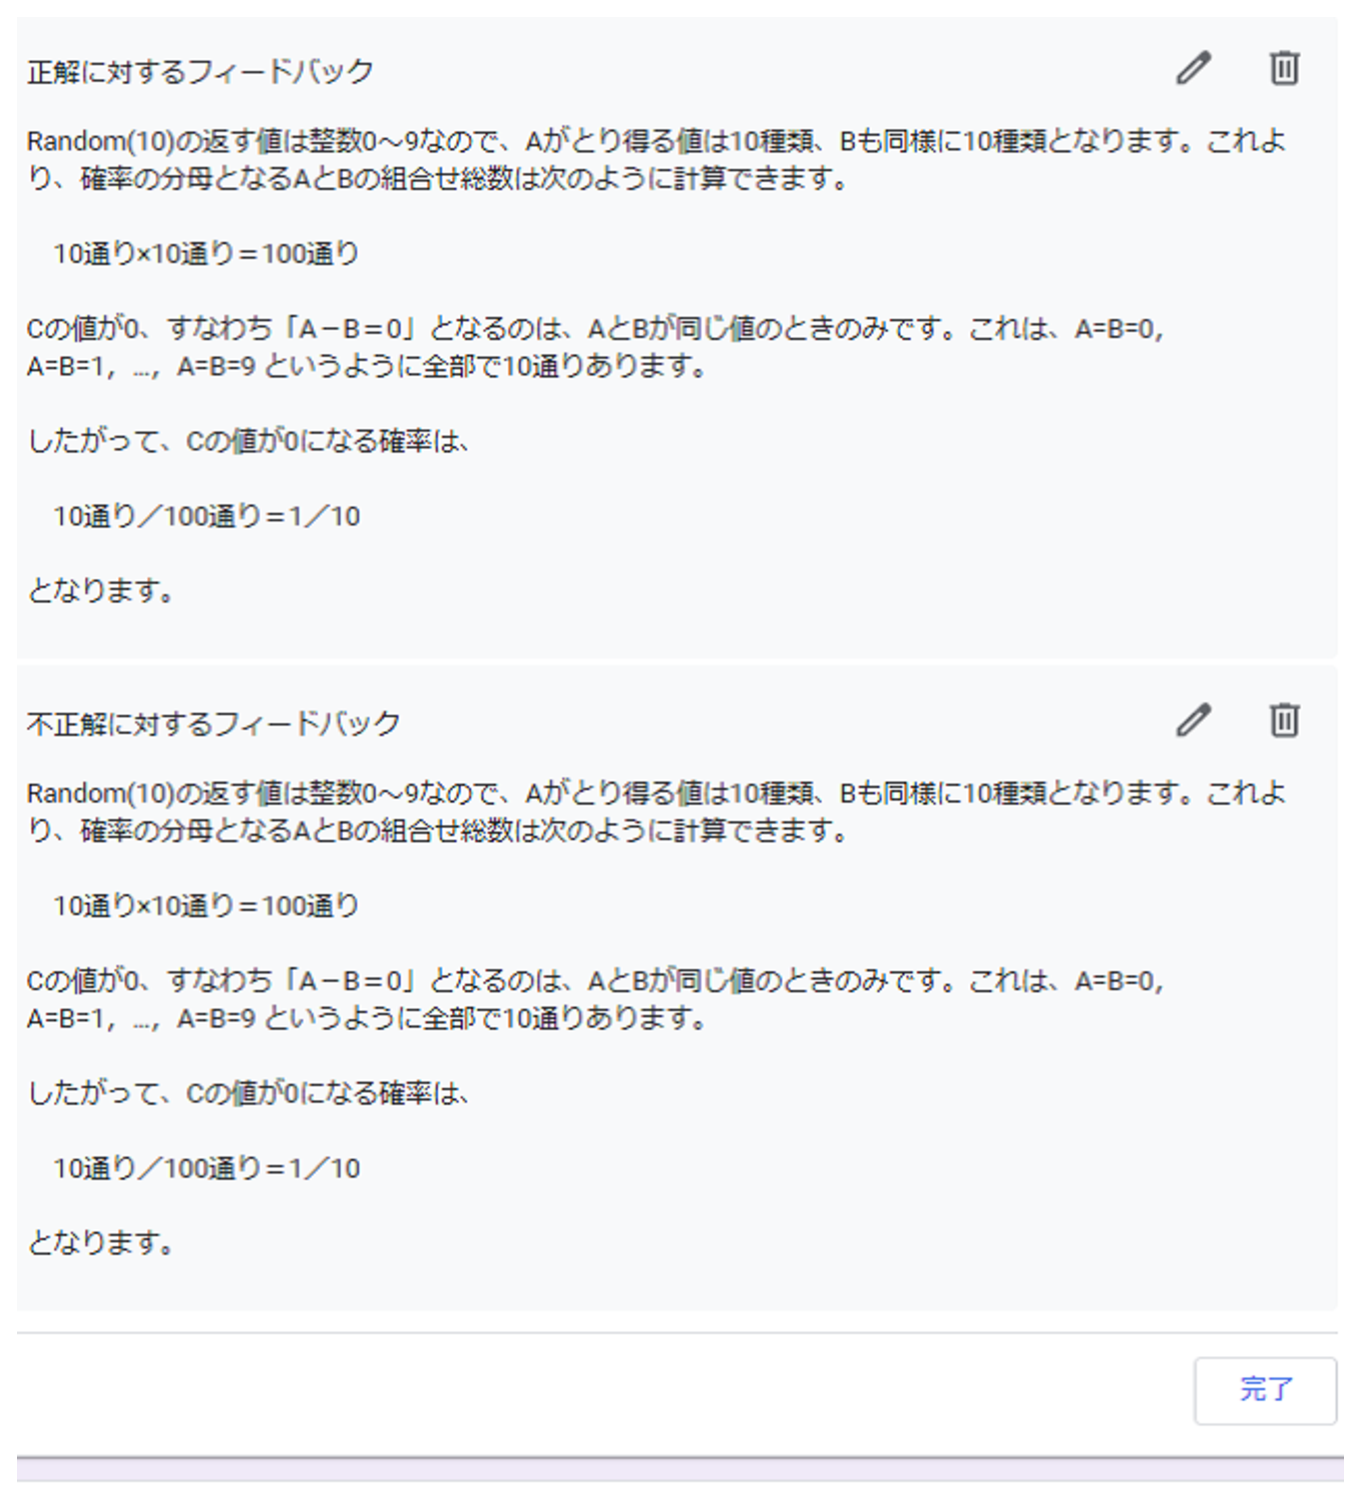
\includegraphics[width=16cm]{img/kyozai1.eps}
\end{center}
\caption{学習教材例1}
\label{fig:kyozai1}
\end{figure}

\begin{figure}[htbp]
\begin{center}
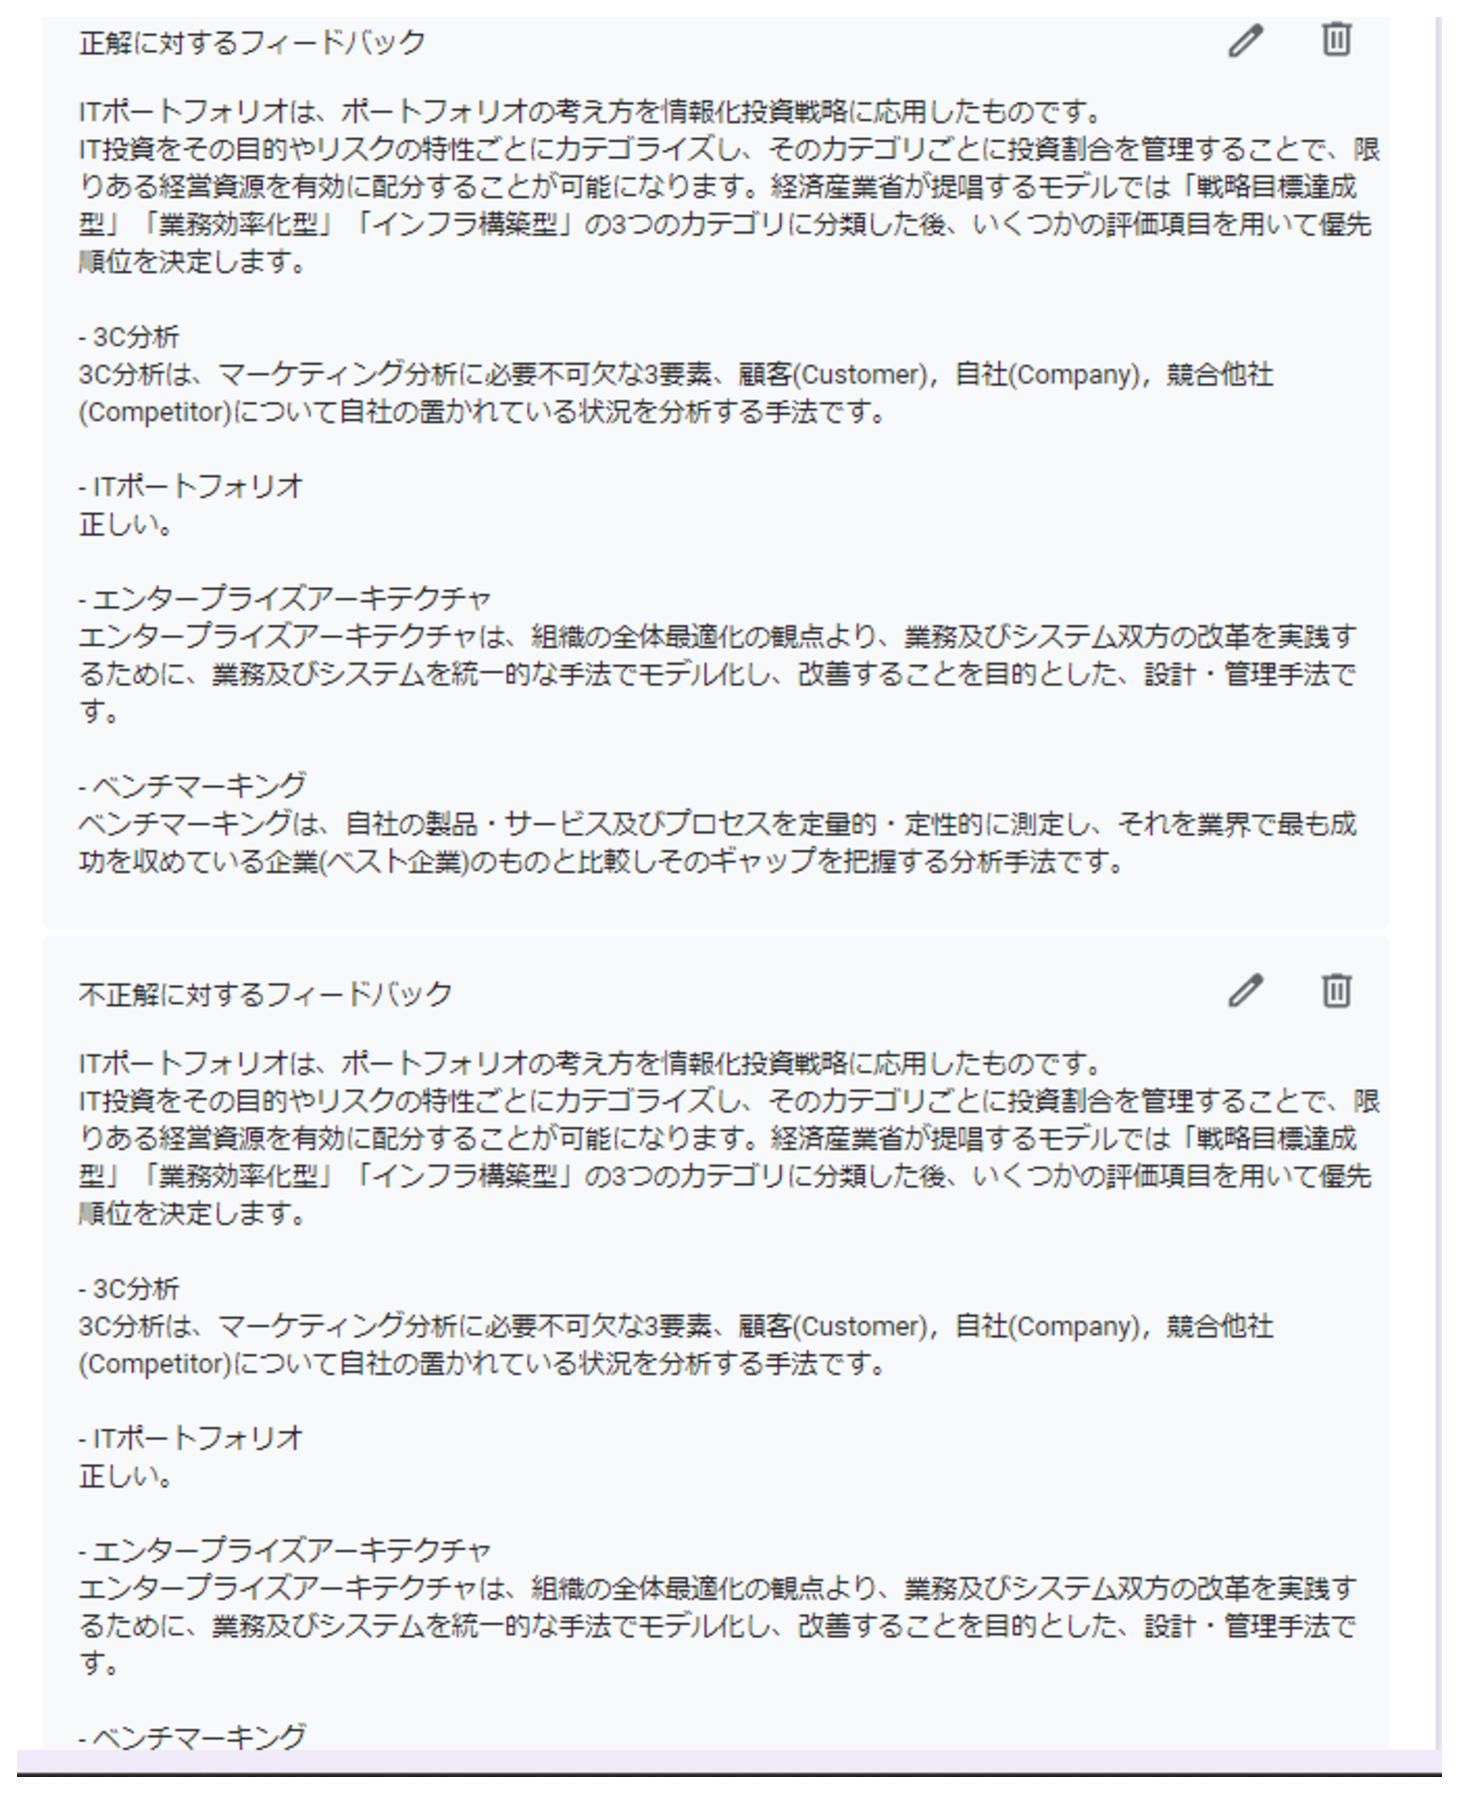
\includegraphics[width=16cm]{img/kyozai2.eps}
\end{center}
\caption{学習教材例2}
\label{fig:kyozai2}
\end{figure}

\subsection{実験手順}
まず,実験対象者16名に対して事前テストを実施した.
次に,事前テストの平均点が均等になるように8名ずつの2グループに分割した.
それぞれのグループをシステム利用者群,システム非利用者群とし,事前テストの結果と学習教材を基に各々のグループには学習目標を立ててもらい学習してもらった.
ただし,学習期間は3日間で合計3時間の学習時間とした.
両グループの学習終了後に実験対象者16名に事後テストを実施した.

\subsection{実験結果}
実験の結果を表\ref{tab:result1}に示す.表\ref{tab:result1}に示されるように,事後テストの点数の標準偏差は小さいため,実験対象者はシステム利用者群とシステム非利用者群ともに一定の水準の学習レベルに到達したと考えられる.
\begin{table}[tb]
    \centering
    \caption{実験結果}
    \label{tab:result1}
    \begin{tabular}{|c|c|c|c|c|c}
    \hline
     & \multicolumn{2}{c|}{事前テスト} & \multicolumn{2}{c|}{事後テスト} \\ \cline{2-5}
     & 平均 & 標準偏差 & 平均 & 標準偏差 \\ \hline
     本システム & 6.875 & 1.726 & 9.000 & 0.925 \\ \hline
     座学 & 6.875 & 1.552 & 7.625 & 1.597 \\ \hline
    \end{tabular}
\end{table}

事前テストと事後テストを受けた実験対象者全体の各問題における正答人数と誤答人数を図\ref{fig:result_jizen},図\ref{fig:result_jigo}に示す.


\begin{figure}[htbp]
\begin{center}
\includegraphics[width=18cm]{img/result_jizen.eps}
\end{center}
\caption{事前テストの全体結果}
\label{fig:result_jizen}
\end{figure}

\begin{figure}[htbp]
\begin{center}
\includegraphics[width=18cm]{img/result_jigo.eps}
\end{center}
\caption{事後テストの全体結果}
\label{fig:result_jigo}
\end{figure}

図\ref{fig:result_jizen}と図\ref{fig:result_jigo}内に示されている通り,誤答の多い問題は正答率が50\%未満の問題に限定すると,事前テストでは2問あったが事後テストではなくなっていることからも,実験対象者は本システムを利用した学習と座学でのみ学習した者たち共に,点数の上昇に限らず,知識を偏りなく習得できていることが確認できる.
また,表\ref{tab:result1}より,座学すなわちシステム非利用者群の平均点が0.75点増えているのに対し,本システム利用者群の平均点は2.125点上昇している.

加えて事前テストと事後テストにおけるt検定の結果を図\ref{fig:tcheck}に示す.
\begin{figure}[htbp]
\begin{center}
\includegraphics[width=18cm]{img/tcheck.eps}
\end{center}
\caption{t検定の結果}
\label{fig:tcheck}
\end{figure}
t検定では帰無仮説を「事前テストと事後テストの平均点は等しい」,対立仮説を「事前テストと事後テストの平均点は等しくない」,有意水準を0.05とした.
図\ref{fig:tcheck}から帰無仮説は棄却され,事前テストと事後テストの平均点は有意に異なることが分かった.
これは表\ref{tab:result1}と併せて考えるとシステム利用者群の平均点がシステム非利用者群と比べ明らかに点数の伸びが高い点から,本システムにおける学習目標設定方法が有意に作用した可能性が挙げられる.

以上の結果から,座学で学習したシステム非利用者群と比較して,本システムを利用して学習したシステム利用者群の方がより高い点数が得られたことが確認できた.

\newpage

\section{本システムの利用評価実験}
最後に本システムの利用評価実験を実施した.
実験対象者は座学と比較した本システムによる学習の有用性検証実験に参加した実験対象者16名全員に対してアンケートによる利用評価実験を行った.
利用評価実験で使用したアンケートは1~5の5段階評価で実施し,最後に自由記述欄を設けた.

アンケート結果を図\ref{fig:ank}に示す.

\begin{figure}[htbp]
\begin{center}
\includegraphics[width=18cm]{img/ank.eps}
\end{center}
\caption{アンケートの結果}
\label{fig:ank}
\end{figure}

アンケート結果から「事前テストの主観的問題難易度はどうでしたか」,「事後テストの主観的問題難易度はどうでしたか」という設問に対して,両群ともに数値が低く,問題難易度が低いと認識していたようである.
「事前テストにおける得点の割合は全体を通してどの程度あると思っていましたか」,「事後テストにおける得点の割合は全体を通してどの程度あると思っていましたか」という設問でも,両群ともに事前テストでは7割程度,事後テストでは8割程度得点出来ていると認識していたようである.
「事前テストの主観的得点と実際に返却された得点はどの程度離れていましたか」という設問に対しても両群ともに同じ割合分ギャップを感じていたようである.
一方「事後テストの主観的得点と実際に返却された得点はどの程度離れていましたか」という設問に対してシステム非利用者群は2.3,システム利用者群は1.5と0.8もの差が開いている.
このことからシステム利用者群はシステム非利用者群と比べて,自分の主観的学習理解度と実際に返却された学習理解度に差がなかったことが表されている.
すなわち,システム利用者の方がシステム非利用者と比べて,学習者自身の学習内容に対する主観的理解度と客観的理解度に差がなかったことが分かった.
この結果から,システム利用者群は正しく自身の学習進行度を理解できていたため,表\ref{tab:result1}で示されたようにシステム非利用者群より事後テストの得点が上昇していたのではと考えられる.

\section{考察}
座学と比較した本システムによる学習の有用性検証実験では,事前テストと事後テストの平均点がシステム利用者群のほうがシステム非利用者群より良い結果となり,t検定からも両群の平均には有意な差があることが分かった.
利用評価実験では,事前事後テストの主観的難易度は両軍ともに同程度と感じていたが,システム非利用者群に比べてシステム利用者群は学習者自身の学習内容に対する主観的理解度と客観的理解度に差がなかったことが分かった.
以上の実験の結果から座学による学習の学習目標設定方法と比べ,本システムを利用した学習目標設定方法のほうが学習者自身が学習内容の構造的理解と,主観的理解度と客観的理解度に差が付きづらいため,より正確な学習目標設定支援を行えることが分かった.
一方,本実験ではシステム非利用者群に対して本システムを用いないコンセプトマップ作成を用いた学習を実施していないため,今後の課題として,本システムを用いないコンセプトマップを用いた学習方法における学習目標設定方法と本システムを用いた学習目標設定方法の比較を実施する必要がある.

%
% 結論
%
\chapter{結論}\label{chap:conclusion}
e ラーニング上で学習するにあたり,自身の学習目標を設定することは,学びを深める手段のうちの一つである.
一方,学習目標を設定するには,自身が学習したい対象の知識を把握している必要がある.
しかし,学習者自身では学習項目を理解していると主観的には考えていても,他人が客観的に判断すると理解できていない場合があり,学習者自身で学習目標を設定することは必ずしも容易ではない.

そこで本研究では,学習目標の設定支援を目的に,学習者の理解度を可視化する,グラフデータベース を用いた学習者理解度可視化システムを開発した.
本システムは e ラーニングで学習している学習者を対象としたシステムで,コンセプトマップ(以下,CMap)を利用して学習者が学習目標を設定する場合に本システムを利用することを想定している.
学習者は指導者が作成した問題を解き,本システムを用いてCMapを作成する.
本システムでは学習者の回答情報からCMapを作成し,学習者は自身が作成したCMapと,システムが生成したCMapを比較することにより,自身の学習理解度を客観的に確認でき,学習目標設定の基準にできる.

開発した本システムを評価するために,学習者が座学における学習目標設定方法による学習と本システムのグラフデータ可視化機能を用いた学習目標設定方法による学習を比較し,有用性を検証するための事前事後テストによる評価実験とアンケートによる利用評価実験を実施した.
座学と比較した本システムによる学習の有用性検証実験では,情報学科の学生と情報学科を卒業した大学院生16名に対して基本情報技術者試験の午前試験を基にした,事前テスト事後テストよる座学と比較した本システムによる学習の有用性を検証した.
結果として,座学すなわちシステム非利用者群の事前テストと事後テストの平均点が0.75 点増えているのに対し,本システム利用者群の平均点は2.125 点上昇していた.
このことから,座学で学習したシステム非利用者群と比較して,本システムを利用して学習したシステム利用者群の方がより高い点数が得られたことが確認できた.

また,本システムの利用評価実験では,システム利用者群はシステム非利用者群と比べて,自分の主観的学習理解度と実際に返却された学習理解度に差がなかったことが表されている.
すなわち,システム利用者の方がシステム非利用者と比べて,学習者自身の学習内容に対する主観的理解度と客観的理解度に差がなかったことが分かった.
この結果から,システム利用者群は正しく自身の学習進行度を理解できていたため,システム非利用者群より事後テストの得点が上昇していたのではと考えられる.

本研究では,e ラーニングにおける学習目標設定支援を目的に,学習者の理解度をCMapで可視化する,グラフデータベースを用いた学習者理解度システムを開発した.
実験の結果座学で学習したグループと比較して,本システムを利用して学習したグループの方がより有意に点数が高いことが確認できた.
このことから本システムは学習目標設定支援が可能である.

%
% 謝辞
%
本研究を遂行するに当たり,熱心な御指導および御鞭撻をいただきました井口信和教授に深く感謝いたします.
また,実験にご協力いただきました被験者の方々に深く感謝いたします.
さらに,ネットワーク研究室の皆様をはじめ,研究活動を支えてくださりました皆様に深く感謝いたします.

%
% 参考文献
%
\include{references}

%
% 付録
%
\appendix
\section{付録について}
本研究で作成したプログラムのソースファイルなどを卒業研究報告書に含めた
い場合は,付録として巻末にまとめておく.

\end{document}